\documentclass{article}

% Reverse-staggered block decoding -- arXiv preprint in the ICLR 2027 layout.
% Uses iclr2027_conference.sty/.bst from the official template (github.com/ICLR/Master-Template).
% Figures are generated by scripts/make_figures.py; scripts/make_upload.py builds the arXiv upload.

\usepackage{iclr2027_conference,times}
% Show the authors. The style then heads every page "Published as a conference paper at ICLR 2027",
% which is replaced by "Preprint" right after \maketitle. For an anonymous submission, remove both.
\iclrfinalcopy

\usepackage[utf8]{inputenc}
\usepackage[T1]{fontenc}
\usepackage{microtype}
\usepackage{amsmath,amssymb,amsthm}
\usepackage{booktabs}
\usepackage{array}
\usepackage{multirow}
\usepackage{makecell}
\usepackage{graphicx}
\usepackage{xcolor}
\usepackage{xspace}
\usepackage{tikz}
\usepackage{pgfplots}
\usepgfplotslibrary{groupplots}
\pgfplotsset{compat=1.17}
\usepackage{url}
\usepackage[colorlinks=true,linkcolor=black!70!blue,citecolor=black!70!blue,urlcolor=black!70!blue]{hyperref}

% Categorical palette used by the generated figures.
\definecolor{cBlue}{HTML}{2A78D6}
\definecolor{cOrange}{HTML}{EB6834}
\definecolor{cAqua}{HTML}{1BAF7A}
\definecolor{cYellow}{HTML}{EDA100}

\newtheorem{proposition}{Proposition}
\theoremstyle{definition}
\newtheorem{definition}{Definition}
\theoremstyle{remark}
\newtheorem{remark}{Remark}

% Schedule names, upright small caps also inside italic text (Times has no italic small caps).
% R_{s,g} and F_s are the general reversed and forward schedules (Section 3.1).
\newcommand{\name}[1]{\textup{\textsc{#1}}}
\newcommand{\sfill}{\name{SkipFill}\xspace}
\newcommand{\rev}{\name{Reverse}\xspace}
\newcommand{\fwd}{\name{Forward}\xspace}
\newcommand{\causal}{\name{Causal}\xspace}
\newcommand{\delayed}{\name{Delayed}\xspace}
\newcommand{\landing}{\name{Landing}\xspace}
\newcommand{\meet}[1]{\name{Meet}$_{#1}$}
\newcommand{\alt}[1]{\name{Alternate}$_{#1}$}
\newcommand{\Rsg}[2]{\mathrm{R}_{#1,#2}}
\newcommand{\Fs}[1]{\mathrm{F}_{#1}}
\newcommand{\blk}{\,{\color{black!45}$\Vert$}\,}
\newcommand{\brk}[1]{\textbf{\color{red!65!black}#1}}
\newcommand{\dmin}{d_{\min}}
\newcommand{\pos}[1]{\max\!\left(0,\,#1\right)}

\title{Write the Seam Last: Which Dependencies\\Should a Block-Parallel Decoder Drop?}
\author{Qiran Li \\ Independent researcher}

\begin{document}
\maketitle
\lhead{Preprint}

\begin{abstract}
Block-parallel decoders speed up language-model generation by starting a block before the previous one is finished, so some dependencies between tokens must be dropped.
Prior work asks how many dependencies a decoder can afford to drop; we ask which ones.
Staggered pipelines write every block left to right and so drop the seam, the dependency between a block's first token and the token just before it.
We show that reordering the tokens inside each block so that the seam is written last leaves both the parallelism and the number of dropped dependencies unchanged, yet moves every dropped dependency at least a block away.
To measure what this buys, we train models that differ only in their attention mask, which separates the information a schedule loses from the cost of learning a non-left-to-right order.
Moved away from the seam, the same dropped dependencies become more than $20\times$ cheaper, and the seam failure largely disappears from samples.
What remains is an ordering cost concentrated at a single token per block, which neither scale nor a block-level plan removes in our experiments; this points to learnability, rather than lost information, as the next bottleneck for block-parallel decoding.
\end{abstract}

% ---------------------------------------------------------------------------
\section{Introduction}
\label{sec:intro}

Language models generate text one token per forward pass, so producing $n$ tokens takes $n$ sequential evaluations of the whole network.
Each evaluation performs little computation per byte of weights it reads, which makes decoding bound by memory bandwidth rather than by arithmetic, and it is the length of this serial chain that sets the time needed to produce a long response~\citep{leviathan2023speculative,chen2023speculative}.
A natural way to cut latency is therefore to emit several tokens per serial step.
Block diffusion~\citep{arriola2025block}, line- and block-parallel language models~\citep{li2026lclm,zhang2026latlm,he2026psf} and pipelined image and video generators~\citep{he2025zipar,ye2025diagonal} all do so, and all pay for it in the same way: tokens produced in the same step cannot condition on each other, so some dependencies between tokens are lost.

Most work on parallel decoding accordingly asks how many dependencies a decoder can drop before quality suffers.
This paper asks which ones it should drop, and finds that the answer matters more than the count.
A common way to keep many tokens in flight is the staggered, or wavefront, pipeline, in which block $t$ starts a fixed number of steps after block $t-1$ and the two then advance together.
Every staggered pipeline we know of writes each block left to right, so the first token of block $t$ is written before the end of block $t-1$ exists, and the dependency it loses is the adjacent one, usually the strongest in the sequence~\citep{wang2025par,li2025refusion}.
Several of these systems identify this \emph{seam} as their main source of quality loss~\citep{he2025zipar,li2026lclm,zhang2026latlm,he2026psf}, and each of their remedies gives something up (Table~\ref{tab:remedies}): waiting for the previous block's tail costs parallelism, repairing the seam afterwards costs extra passes, and letting a block read ahead into the next gives up block-by-block commitment.

\begin{figure}[t]
  \centering
  \resizebox{\textwidth}{!}{% Generated by scripts/make_figures.py -- do not edit by hand.
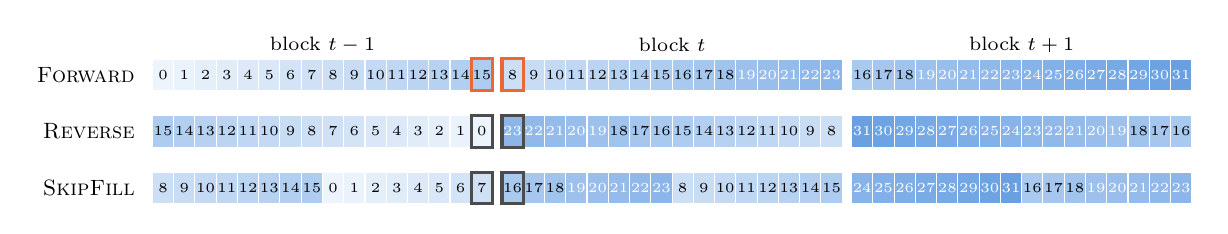
\begin{tikzpicture}[x=1cm, y=1cm, font=\tiny]
\node[anchor=east, font=\footnotesize] at (-0.1,0.20) {\textsc{Forward}};
\draw[fill=cBlue!8, draw=white, line width=0.4pt] (0.00,0.00) rectangle ++(0.27,0.40) node[pos=0.5, text=black] {0};
\draw[fill=cBlue!10, draw=white, line width=0.4pt] (0.27,0.00) rectangle ++(0.27,0.40) node[pos=0.5, text=black] {1};
\draw[fill=cBlue!12, draw=white, line width=0.4pt] (0.54,0.00) rectangle ++(0.27,0.40) node[pos=0.5, text=black] {2};
\draw[fill=cBlue!14, draw=white, line width=0.4pt] (0.81,0.00) rectangle ++(0.27,0.40) node[pos=0.5, text=black] {3};
\draw[fill=cBlue!16, draw=white, line width=0.4pt] (1.08,0.00) rectangle ++(0.27,0.40) node[pos=0.5, text=black] {4};
\draw[fill=cBlue!18, draw=white, line width=0.4pt] (1.35,0.00) rectangle ++(0.27,0.40) node[pos=0.5, text=black] {5};
\draw[fill=cBlue!20, draw=white, line width=0.4pt] (1.62,0.00) rectangle ++(0.27,0.40) node[pos=0.5, text=black] {6};
\draw[fill=cBlue!22, draw=white, line width=0.4pt] (1.89,0.00) rectangle ++(0.27,0.40) node[pos=0.5, text=black] {7};
\draw[fill=cBlue!24, draw=white, line width=0.4pt] (2.16,0.00) rectangle ++(0.27,0.40) node[pos=0.5, text=black] {8};
\draw[fill=cBlue!26, draw=white, line width=0.4pt] (2.43,0.00) rectangle ++(0.27,0.40) node[pos=0.5, text=black] {9};
\draw[fill=cBlue!28, draw=white, line width=0.4pt] (2.70,0.00) rectangle ++(0.27,0.40) node[pos=0.5, text=black] {10};
\draw[fill=cBlue!30, draw=white, line width=0.4pt] (2.97,0.00) rectangle ++(0.27,0.40) node[pos=0.5, text=black] {11};
\draw[fill=cBlue!32, draw=white, line width=0.4pt] (3.24,0.00) rectangle ++(0.27,0.40) node[pos=0.5, text=black] {12};
\draw[fill=cBlue!34, draw=white, line width=0.4pt] (3.51,0.00) rectangle ++(0.27,0.40) node[pos=0.5, text=black] {13};
\draw[fill=cBlue!36, draw=white, line width=0.4pt] (3.78,0.00) rectangle ++(0.27,0.40) node[pos=0.5, text=black] {14};
\draw[fill=cBlue!38, draw=white, line width=0.4pt] (4.05,0.00) rectangle ++(0.27,0.40) node[pos=0.5, text=black] {15};
\draw[fill=cBlue!24, draw=white, line width=0.4pt] (4.44,0.00) rectangle ++(0.27,0.40) node[pos=0.5, text=black] {8};
\draw[fill=cBlue!26, draw=white, line width=0.4pt] (4.71,0.00) rectangle ++(0.27,0.40) node[pos=0.5, text=black] {9};
\draw[fill=cBlue!28, draw=white, line width=0.4pt] (4.98,0.00) rectangle ++(0.27,0.40) node[pos=0.5, text=black] {10};
\draw[fill=cBlue!30, draw=white, line width=0.4pt] (5.25,0.00) rectangle ++(0.27,0.40) node[pos=0.5, text=black] {11};
\draw[fill=cBlue!32, draw=white, line width=0.4pt] (5.52,0.00) rectangle ++(0.27,0.40) node[pos=0.5, text=black] {12};
\draw[fill=cBlue!34, draw=white, line width=0.4pt] (5.79,0.00) rectangle ++(0.27,0.40) node[pos=0.5, text=black] {13};
\draw[fill=cBlue!36, draw=white, line width=0.4pt] (6.06,0.00) rectangle ++(0.27,0.40) node[pos=0.5, text=black] {14};
\draw[fill=cBlue!38, draw=white, line width=0.4pt] (6.33,0.00) rectangle ++(0.27,0.40) node[pos=0.5, text=black] {15};
\draw[fill=cBlue!40, draw=white, line width=0.4pt] (6.60,0.00) rectangle ++(0.27,0.40) node[pos=0.5, text=black] {16};
\draw[fill=cBlue!42, draw=white, line width=0.4pt] (6.87,0.00) rectangle ++(0.27,0.40) node[pos=0.5, text=black] {17};
\draw[fill=cBlue!44, draw=white, line width=0.4pt] (7.14,0.00) rectangle ++(0.27,0.40) node[pos=0.5, text=black] {18};
\draw[fill=cBlue!46, draw=white, line width=0.4pt] (7.41,0.00) rectangle ++(0.27,0.40) node[pos=0.5, text=white] {19};
\draw[fill=cBlue!48, draw=white, line width=0.4pt] (7.68,0.00) rectangle ++(0.27,0.40) node[pos=0.5, text=white] {20};
\draw[fill=cBlue!50, draw=white, line width=0.4pt] (7.95,0.00) rectangle ++(0.27,0.40) node[pos=0.5, text=white] {21};
\draw[fill=cBlue!52, draw=white, line width=0.4pt] (8.22,0.00) rectangle ++(0.27,0.40) node[pos=0.5, text=white] {22};
\draw[fill=cBlue!54, draw=white, line width=0.4pt] (8.49,0.00) rectangle ++(0.27,0.40) node[pos=0.5, text=white] {23};
\draw[fill=cBlue!40, draw=white, line width=0.4pt] (8.88,0.00) rectangle ++(0.27,0.40) node[pos=0.5, text=black] {16};
\draw[fill=cBlue!42, draw=white, line width=0.4pt] (9.15,0.00) rectangle ++(0.27,0.40) node[pos=0.5, text=black] {17};
\draw[fill=cBlue!44, draw=white, line width=0.4pt] (9.42,0.00) rectangle ++(0.27,0.40) node[pos=0.5, text=black] {18};
\draw[fill=cBlue!46, draw=white, line width=0.4pt] (9.69,0.00) rectangle ++(0.27,0.40) node[pos=0.5, text=white] {19};
\draw[fill=cBlue!48, draw=white, line width=0.4pt] (9.96,0.00) rectangle ++(0.27,0.40) node[pos=0.5, text=white] {20};
\draw[fill=cBlue!50, draw=white, line width=0.4pt] (10.23,0.00) rectangle ++(0.27,0.40) node[pos=0.5, text=white] {21};
\draw[fill=cBlue!52, draw=white, line width=0.4pt] (10.50,0.00) rectangle ++(0.27,0.40) node[pos=0.5, text=white] {22};
\draw[fill=cBlue!54, draw=white, line width=0.4pt] (10.77,0.00) rectangle ++(0.27,0.40) node[pos=0.5, text=white] {23};
\draw[fill=cBlue!56, draw=white, line width=0.4pt] (11.04,0.00) rectangle ++(0.27,0.40) node[pos=0.5, text=white] {24};
\draw[fill=cBlue!58, draw=white, line width=0.4pt] (11.31,0.00) rectangle ++(0.27,0.40) node[pos=0.5, text=white] {25};
\draw[fill=cBlue!60, draw=white, line width=0.4pt] (11.58,0.00) rectangle ++(0.27,0.40) node[pos=0.5, text=white] {26};
\draw[fill=cBlue!62, draw=white, line width=0.4pt] (11.85,0.00) rectangle ++(0.27,0.40) node[pos=0.5, text=white] {27};
\draw[fill=cBlue!64, draw=white, line width=0.4pt] (12.12,0.00) rectangle ++(0.27,0.40) node[pos=0.5, text=white] {28};
\draw[fill=cBlue!66, draw=white, line width=0.4pt] (12.39,0.00) rectangle ++(0.27,0.40) node[pos=0.5, text=white] {29};
\draw[fill=cBlue!68, draw=white, line width=0.4pt] (12.66,0.00) rectangle ++(0.27,0.40) node[pos=0.5, text=white] {30};
\draw[fill=cBlue!70, draw=white, line width=0.4pt] (12.93,0.00) rectangle ++(0.27,0.40) node[pos=0.5, text=white] {31};
\draw[cOrange, line width=1.1pt] (4.05,0.00) rectangle ++(0.27,0.40);\draw[cOrange, line width=1.1pt] (4.44,0.00) rectangle ++(0.27,0.40);
\node[anchor=east, font=\footnotesize] at (-0.1,-0.52) {\textsc{Reverse}};
\draw[fill=cBlue!38, draw=white, line width=0.4pt] (0.00,-0.72) rectangle ++(0.27,0.40) node[pos=0.5, text=black] {15};
\draw[fill=cBlue!36, draw=white, line width=0.4pt] (0.27,-0.72) rectangle ++(0.27,0.40) node[pos=0.5, text=black] {14};
\draw[fill=cBlue!34, draw=white, line width=0.4pt] (0.54,-0.72) rectangle ++(0.27,0.40) node[pos=0.5, text=black] {13};
\draw[fill=cBlue!32, draw=white, line width=0.4pt] (0.81,-0.72) rectangle ++(0.27,0.40) node[pos=0.5, text=black] {12};
\draw[fill=cBlue!30, draw=white, line width=0.4pt] (1.08,-0.72) rectangle ++(0.27,0.40) node[pos=0.5, text=black] {11};
\draw[fill=cBlue!28, draw=white, line width=0.4pt] (1.35,-0.72) rectangle ++(0.27,0.40) node[pos=0.5, text=black] {10};
\draw[fill=cBlue!26, draw=white, line width=0.4pt] (1.62,-0.72) rectangle ++(0.27,0.40) node[pos=0.5, text=black] {9};
\draw[fill=cBlue!24, draw=white, line width=0.4pt] (1.89,-0.72) rectangle ++(0.27,0.40) node[pos=0.5, text=black] {8};
\draw[fill=cBlue!22, draw=white, line width=0.4pt] (2.16,-0.72) rectangle ++(0.27,0.40) node[pos=0.5, text=black] {7};
\draw[fill=cBlue!20, draw=white, line width=0.4pt] (2.43,-0.72) rectangle ++(0.27,0.40) node[pos=0.5, text=black] {6};
\draw[fill=cBlue!18, draw=white, line width=0.4pt] (2.70,-0.72) rectangle ++(0.27,0.40) node[pos=0.5, text=black] {5};
\draw[fill=cBlue!16, draw=white, line width=0.4pt] (2.97,-0.72) rectangle ++(0.27,0.40) node[pos=0.5, text=black] {4};
\draw[fill=cBlue!14, draw=white, line width=0.4pt] (3.24,-0.72) rectangle ++(0.27,0.40) node[pos=0.5, text=black] {3};
\draw[fill=cBlue!12, draw=white, line width=0.4pt] (3.51,-0.72) rectangle ++(0.27,0.40) node[pos=0.5, text=black] {2};
\draw[fill=cBlue!10, draw=white, line width=0.4pt] (3.78,-0.72) rectangle ++(0.27,0.40) node[pos=0.5, text=black] {1};
\draw[fill=cBlue!8, draw=white, line width=0.4pt] (4.05,-0.72) rectangle ++(0.27,0.40) node[pos=0.5, text=black] {0};
\draw[fill=cBlue!54, draw=white, line width=0.4pt] (4.44,-0.72) rectangle ++(0.27,0.40) node[pos=0.5, text=white] {23};
\draw[fill=cBlue!52, draw=white, line width=0.4pt] (4.71,-0.72) rectangle ++(0.27,0.40) node[pos=0.5, text=white] {22};
\draw[fill=cBlue!50, draw=white, line width=0.4pt] (4.98,-0.72) rectangle ++(0.27,0.40) node[pos=0.5, text=white] {21};
\draw[fill=cBlue!48, draw=white, line width=0.4pt] (5.25,-0.72) rectangle ++(0.27,0.40) node[pos=0.5, text=white] {20};
\draw[fill=cBlue!46, draw=white, line width=0.4pt] (5.52,-0.72) rectangle ++(0.27,0.40) node[pos=0.5, text=white] {19};
\draw[fill=cBlue!44, draw=white, line width=0.4pt] (5.79,-0.72) rectangle ++(0.27,0.40) node[pos=0.5, text=black] {18};
\draw[fill=cBlue!42, draw=white, line width=0.4pt] (6.06,-0.72) rectangle ++(0.27,0.40) node[pos=0.5, text=black] {17};
\draw[fill=cBlue!40, draw=white, line width=0.4pt] (6.33,-0.72) rectangle ++(0.27,0.40) node[pos=0.5, text=black] {16};
\draw[fill=cBlue!38, draw=white, line width=0.4pt] (6.60,-0.72) rectangle ++(0.27,0.40) node[pos=0.5, text=black] {15};
\draw[fill=cBlue!36, draw=white, line width=0.4pt] (6.87,-0.72) rectangle ++(0.27,0.40) node[pos=0.5, text=black] {14};
\draw[fill=cBlue!34, draw=white, line width=0.4pt] (7.14,-0.72) rectangle ++(0.27,0.40) node[pos=0.5, text=black] {13};
\draw[fill=cBlue!32, draw=white, line width=0.4pt] (7.41,-0.72) rectangle ++(0.27,0.40) node[pos=0.5, text=black] {12};
\draw[fill=cBlue!30, draw=white, line width=0.4pt] (7.68,-0.72) rectangle ++(0.27,0.40) node[pos=0.5, text=black] {11};
\draw[fill=cBlue!28, draw=white, line width=0.4pt] (7.95,-0.72) rectangle ++(0.27,0.40) node[pos=0.5, text=black] {10};
\draw[fill=cBlue!26, draw=white, line width=0.4pt] (8.22,-0.72) rectangle ++(0.27,0.40) node[pos=0.5, text=black] {9};
\draw[fill=cBlue!24, draw=white, line width=0.4pt] (8.49,-0.72) rectangle ++(0.27,0.40) node[pos=0.5, text=black] {8};
\draw[fill=cBlue!70, draw=white, line width=0.4pt] (8.88,-0.72) rectangle ++(0.27,0.40) node[pos=0.5, text=white] {31};
\draw[fill=cBlue!68, draw=white, line width=0.4pt] (9.15,-0.72) rectangle ++(0.27,0.40) node[pos=0.5, text=white] {30};
\draw[fill=cBlue!66, draw=white, line width=0.4pt] (9.42,-0.72) rectangle ++(0.27,0.40) node[pos=0.5, text=white] {29};
\draw[fill=cBlue!64, draw=white, line width=0.4pt] (9.69,-0.72) rectangle ++(0.27,0.40) node[pos=0.5, text=white] {28};
\draw[fill=cBlue!62, draw=white, line width=0.4pt] (9.96,-0.72) rectangle ++(0.27,0.40) node[pos=0.5, text=white] {27};
\draw[fill=cBlue!60, draw=white, line width=0.4pt] (10.23,-0.72) rectangle ++(0.27,0.40) node[pos=0.5, text=white] {26};
\draw[fill=cBlue!58, draw=white, line width=0.4pt] (10.50,-0.72) rectangle ++(0.27,0.40) node[pos=0.5, text=white] {25};
\draw[fill=cBlue!56, draw=white, line width=0.4pt] (10.77,-0.72) rectangle ++(0.27,0.40) node[pos=0.5, text=white] {24};
\draw[fill=cBlue!54, draw=white, line width=0.4pt] (11.04,-0.72) rectangle ++(0.27,0.40) node[pos=0.5, text=white] {23};
\draw[fill=cBlue!52, draw=white, line width=0.4pt] (11.31,-0.72) rectangle ++(0.27,0.40) node[pos=0.5, text=white] {22};
\draw[fill=cBlue!50, draw=white, line width=0.4pt] (11.58,-0.72) rectangle ++(0.27,0.40) node[pos=0.5, text=white] {21};
\draw[fill=cBlue!48, draw=white, line width=0.4pt] (11.85,-0.72) rectangle ++(0.27,0.40) node[pos=0.5, text=white] {20};
\draw[fill=cBlue!46, draw=white, line width=0.4pt] (12.12,-0.72) rectangle ++(0.27,0.40) node[pos=0.5, text=white] {19};
\draw[fill=cBlue!44, draw=white, line width=0.4pt] (12.39,-0.72) rectangle ++(0.27,0.40) node[pos=0.5, text=black] {18};
\draw[fill=cBlue!42, draw=white, line width=0.4pt] (12.66,-0.72) rectangle ++(0.27,0.40) node[pos=0.5, text=black] {17};
\draw[fill=cBlue!40, draw=white, line width=0.4pt] (12.93,-0.72) rectangle ++(0.27,0.40) node[pos=0.5, text=black] {16};
\draw[black!70, line width=1.1pt] (4.05,-0.72) rectangle ++(0.27,0.40);\draw[black!70, line width=1.1pt] (4.44,-0.72) rectangle ++(0.27,0.40);
\node[anchor=east, font=\footnotesize] at (-0.1,-1.24) {\textsc{SkipFill}};
\draw[fill=cBlue!24, draw=white, line width=0.4pt] (0.00,-1.44) rectangle ++(0.27,0.40) node[pos=0.5, text=black] {8};
\draw[fill=cBlue!26, draw=white, line width=0.4pt] (0.27,-1.44) rectangle ++(0.27,0.40) node[pos=0.5, text=black] {9};
\draw[fill=cBlue!28, draw=white, line width=0.4pt] (0.54,-1.44) rectangle ++(0.27,0.40) node[pos=0.5, text=black] {10};
\draw[fill=cBlue!30, draw=white, line width=0.4pt] (0.81,-1.44) rectangle ++(0.27,0.40) node[pos=0.5, text=black] {11};
\draw[fill=cBlue!32, draw=white, line width=0.4pt] (1.08,-1.44) rectangle ++(0.27,0.40) node[pos=0.5, text=black] {12};
\draw[fill=cBlue!34, draw=white, line width=0.4pt] (1.35,-1.44) rectangle ++(0.27,0.40) node[pos=0.5, text=black] {13};
\draw[fill=cBlue!36, draw=white, line width=0.4pt] (1.62,-1.44) rectangle ++(0.27,0.40) node[pos=0.5, text=black] {14};
\draw[fill=cBlue!38, draw=white, line width=0.4pt] (1.89,-1.44) rectangle ++(0.27,0.40) node[pos=0.5, text=black] {15};
\draw[fill=cBlue!8, draw=white, line width=0.4pt] (2.16,-1.44) rectangle ++(0.27,0.40) node[pos=0.5, text=black] {0};
\draw[fill=cBlue!10, draw=white, line width=0.4pt] (2.43,-1.44) rectangle ++(0.27,0.40) node[pos=0.5, text=black] {1};
\draw[fill=cBlue!12, draw=white, line width=0.4pt] (2.70,-1.44) rectangle ++(0.27,0.40) node[pos=0.5, text=black] {2};
\draw[fill=cBlue!14, draw=white, line width=0.4pt] (2.97,-1.44) rectangle ++(0.27,0.40) node[pos=0.5, text=black] {3};
\draw[fill=cBlue!16, draw=white, line width=0.4pt] (3.24,-1.44) rectangle ++(0.27,0.40) node[pos=0.5, text=black] {4};
\draw[fill=cBlue!18, draw=white, line width=0.4pt] (3.51,-1.44) rectangle ++(0.27,0.40) node[pos=0.5, text=black] {5};
\draw[fill=cBlue!20, draw=white, line width=0.4pt] (3.78,-1.44) rectangle ++(0.27,0.40) node[pos=0.5, text=black] {6};
\draw[fill=cBlue!22, draw=white, line width=0.4pt] (4.05,-1.44) rectangle ++(0.27,0.40) node[pos=0.5, text=black] {7};
\draw[fill=cBlue!40, draw=white, line width=0.4pt] (4.44,-1.44) rectangle ++(0.27,0.40) node[pos=0.5, text=black] {16};
\draw[fill=cBlue!42, draw=white, line width=0.4pt] (4.71,-1.44) rectangle ++(0.27,0.40) node[pos=0.5, text=black] {17};
\draw[fill=cBlue!44, draw=white, line width=0.4pt] (4.98,-1.44) rectangle ++(0.27,0.40) node[pos=0.5, text=black] {18};
\draw[fill=cBlue!46, draw=white, line width=0.4pt] (5.25,-1.44) rectangle ++(0.27,0.40) node[pos=0.5, text=white] {19};
\draw[fill=cBlue!48, draw=white, line width=0.4pt] (5.52,-1.44) rectangle ++(0.27,0.40) node[pos=0.5, text=white] {20};
\draw[fill=cBlue!50, draw=white, line width=0.4pt] (5.79,-1.44) rectangle ++(0.27,0.40) node[pos=0.5, text=white] {21};
\draw[fill=cBlue!52, draw=white, line width=0.4pt] (6.06,-1.44) rectangle ++(0.27,0.40) node[pos=0.5, text=white] {22};
\draw[fill=cBlue!54, draw=white, line width=0.4pt] (6.33,-1.44) rectangle ++(0.27,0.40) node[pos=0.5, text=white] {23};
\draw[fill=cBlue!24, draw=white, line width=0.4pt] (6.60,-1.44) rectangle ++(0.27,0.40) node[pos=0.5, text=black] {8};
\draw[fill=cBlue!26, draw=white, line width=0.4pt] (6.87,-1.44) rectangle ++(0.27,0.40) node[pos=0.5, text=black] {9};
\draw[fill=cBlue!28, draw=white, line width=0.4pt] (7.14,-1.44) rectangle ++(0.27,0.40) node[pos=0.5, text=black] {10};
\draw[fill=cBlue!30, draw=white, line width=0.4pt] (7.41,-1.44) rectangle ++(0.27,0.40) node[pos=0.5, text=black] {11};
\draw[fill=cBlue!32, draw=white, line width=0.4pt] (7.68,-1.44) rectangle ++(0.27,0.40) node[pos=0.5, text=black] {12};
\draw[fill=cBlue!34, draw=white, line width=0.4pt] (7.95,-1.44) rectangle ++(0.27,0.40) node[pos=0.5, text=black] {13};
\draw[fill=cBlue!36, draw=white, line width=0.4pt] (8.22,-1.44) rectangle ++(0.27,0.40) node[pos=0.5, text=black] {14};
\draw[fill=cBlue!38, draw=white, line width=0.4pt] (8.49,-1.44) rectangle ++(0.27,0.40) node[pos=0.5, text=black] {15};
\draw[fill=cBlue!56, draw=white, line width=0.4pt] (8.88,-1.44) rectangle ++(0.27,0.40) node[pos=0.5, text=white] {24};
\draw[fill=cBlue!58, draw=white, line width=0.4pt] (9.15,-1.44) rectangle ++(0.27,0.40) node[pos=0.5, text=white] {25};
\draw[fill=cBlue!60, draw=white, line width=0.4pt] (9.42,-1.44) rectangle ++(0.27,0.40) node[pos=0.5, text=white] {26};
\draw[fill=cBlue!62, draw=white, line width=0.4pt] (9.69,-1.44) rectangle ++(0.27,0.40) node[pos=0.5, text=white] {27};
\draw[fill=cBlue!64, draw=white, line width=0.4pt] (9.96,-1.44) rectangle ++(0.27,0.40) node[pos=0.5, text=white] {28};
\draw[fill=cBlue!66, draw=white, line width=0.4pt] (10.23,-1.44) rectangle ++(0.27,0.40) node[pos=0.5, text=white] {29};
\draw[fill=cBlue!68, draw=white, line width=0.4pt] (10.50,-1.44) rectangle ++(0.27,0.40) node[pos=0.5, text=white] {30};
\draw[fill=cBlue!70, draw=white, line width=0.4pt] (10.77,-1.44) rectangle ++(0.27,0.40) node[pos=0.5, text=white] {31};
\draw[fill=cBlue!40, draw=white, line width=0.4pt] (11.04,-1.44) rectangle ++(0.27,0.40) node[pos=0.5, text=black] {16};
\draw[fill=cBlue!42, draw=white, line width=0.4pt] (11.31,-1.44) rectangle ++(0.27,0.40) node[pos=0.5, text=black] {17};
\draw[fill=cBlue!44, draw=white, line width=0.4pt] (11.58,-1.44) rectangle ++(0.27,0.40) node[pos=0.5, text=black] {18};
\draw[fill=cBlue!46, draw=white, line width=0.4pt] (11.85,-1.44) rectangle ++(0.27,0.40) node[pos=0.5, text=white] {19};
\draw[fill=cBlue!48, draw=white, line width=0.4pt] (12.12,-1.44) rectangle ++(0.27,0.40) node[pos=0.5, text=white] {20};
\draw[fill=cBlue!50, draw=white, line width=0.4pt] (12.39,-1.44) rectangle ++(0.27,0.40) node[pos=0.5, text=white] {21};
\draw[fill=cBlue!52, draw=white, line width=0.4pt] (12.66,-1.44) rectangle ++(0.27,0.40) node[pos=0.5, text=white] {22};
\draw[fill=cBlue!54, draw=white, line width=0.4pt] (12.93,-1.44) rectangle ++(0.27,0.40) node[pos=0.5, text=white] {23};
\draw[black!70, line width=1.1pt] (4.05,-1.44) rectangle ++(0.27,0.40);\draw[black!70, line width=1.1pt] (4.44,-1.44) rectangle ++(0.27,0.40);
\node[font=\scriptsize] at (2.16,0.58) {block $t-1$};
\node[font=\scriptsize] at (6.60,0.58) {block $t$};
\node[font=\scriptsize] at (11.04,0.58) {block $t+1$};
\end{tikzpicture}
}
  \par\medskip
  % Generated by scripts/make_figures.py -- do not edit by hand.
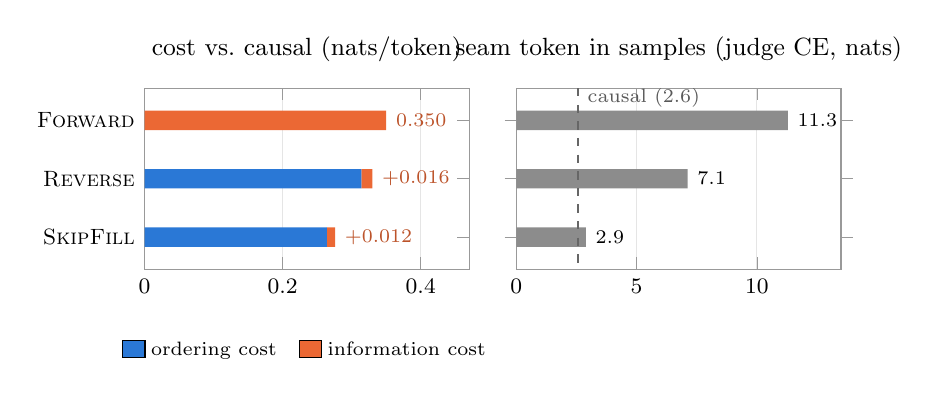
\begin{tikzpicture}
\begin{groupplot}[group style={group size=2 by 1, horizontal sep=0.6cm},
  scale only axis, width=0.34\textwidth, height=2.3cm, ymin=0.45, ymax=3.55, ytick={1,2,3}, y dir=reverse,
  axis line style={black!40}, tick style={black!40}, xmajorgrids, grid style={black!10},
  tick label style={font=\footnotesize}, title style={font=\small}]
\nextgroupplot[xbar stacked, bar width=7pt, xmin=0, xmax=0.47, yticklabels={\textsc{Forward},\textsc{Reverse},\textsc{SkipFill}},
  title={cost vs.\ causal (nats/token)}, legend columns=2, legend cell align=left,
  legend style={font=\scriptsize, draw=none, at={(0.5,-0.34)}, anchor=north,
    /tikz/every even column/.append style={column sep=6pt}}]
\addplot[fill=cBlue, draw=none] coordinates {(0.000,1) (0.314,2) (0.264,3)};
\addlegendentry{ordering cost}
\addplot[fill=cOrange, draw=none] coordinates {(0.350,1) (0.016,2) (0.012,3)};
\addlegendentry{information cost}
\node[anchor=west, font=\scriptsize, text=cOrange!80!black] at (axis cs:0.350,1) {0.350};
\node[anchor=west, font=\scriptsize, text=cOrange!80!black] at (axis cs:0.330,2) {+0.016};
\node[anchor=west, font=\scriptsize, text=cOrange!80!black] at (axis cs:0.276,3) {+0.012};
\nextgroupplot[xbar, bar width=7pt, xmin=0, xmax=13.5, yticklabels={},
  title={seam token in samples (judge CE, nats)}, point meta=x, nodes near coords align={horizontal},
  nodes near coords={\pgfmathprintnumber[fixed,precision=1]{\pgfplotspointmeta}},
  every node near coord/.append style={font=\scriptsize}]
\addplot[fill=black!45, draw=none] coordinates {(11.29,1) (7.12,2) (2.89,3)};
\draw[black!60, dashed, line width=0.8pt] (axis cs:2.56,0.45) -- (axis cs:2.56,3.55);
\node[anchor=west, font=\scriptsize, text=black!65] at (axis cs:2.56,0.62) {causal (2.6)};
\end{groupplot}
\end{tikzpicture}

  \caption{\textbf{Same number of dropped pairs, different placement.}
  Top: generation step of each token for three blocks of $L=16$ under three schedules with the same stagger $s=8$ (darker is later). Outlined cells are the seam, the last token of block $t-1$ and the first of block $t$. \fwd writes the seam token at step 8, before its left neighbour (step 15), so the seam is dropped (orange); \rev and \sfill write it after the previous block is complete (black). All three drop 216 token pairs per window.
  Bottom left: cost over a causal model, split into ordering cost (that of the same write order without staggering, which drops nothing) and information cost (the rest); means of 3 seeds.
  Bottom right: cross-entropy of the seam token in samples from the seed-42 models, under an independently trained causal judge.}
  \label{fig:teaser}
\end{figure}

We propose a remedy that gives up none of these: \textbf{write the seam last}.
If the tokens inside each block are ordered so that a block's head is written after its predecessor's tail, the seam token can read that tail whatever else the schedule does, and because only the order inside a block changes, the parallelism stays the same, no passes are added and nothing reads ahead.
We study two schedules built on this rule (Figure~\ref{fig:teaser}, top).
\rev writes each block from its last token to its first, while \sfill writes the right half of a block first and fills in the left half one stagger later, once both of its neighbours exist.
At the same stagger, both drop exactly as many token pairs as forward staggering, yet every pair they drop is at least a block apart.

Whether this helps is not obvious, because reordering a block changes two things at once: it drops different pairs, and it asks the model to learn a non-left-to-right order.
The chain rule guarantees that the second change loses no information, but a finite model may still find the new order harder to learn.
We separate the two effects with a \emph{mask-only} testbed, in which models differ only in their attention mask, and split each schedule's excess cross-entropy into an \emph{information cost} and an \emph{ordering cost}.
The split gives a clear answer (Figure~\ref{fig:teaser}, bottom).
Moved away from the seam, the same dropped pairs become more than twenty times cheaper, and in samples the seam token goes from by far the least natural token of a block to about as natural as in causal text.
What \sfill still pays is almost entirely ordering cost, concentrated at the one token per block that must be predicted ahead of everything it can see, and in our experiments neither longer training, a larger model, more data nor a block-level plan removes it.

\paragraph{Scope.}
We study decoders that commit tokens without verification, such as block-latent and block-diffusion pipelines.
Draft-and-verify methods such as speculative decoding~\citep{leviathan2023speculative,chen2023speculative} keep the causal distribution and answer a different question, so the two lines of work are complementary.
Our experiments are small and controlled by design: TinyStories~\citep{eldan2023tinystories}, models of 7.2M and 31.5M parameters, and parallelism counted in serial steps, a hardware-independent quantity, rather than in wall-clock time (\S\ref{sec:limitations}).

\begin{table}[t]
  \centering
  \caption{How block pipelines handle the seam. ``Causal'': no token reads a later block, so each block can be committed once written. Representative examples: waiting for the tail~\citep{zhang2026latlm}, reading ahead~\citep{he2026psf} and repairing afterwards~\citep{tsou2026tecop,tian2026flowblock,ren2026asynclane}.}
  \label{tab:remedies}
  \small
  \begin{tabular}{lccc>{\raggedright\arraybackslash}p{4.6cm}}
    \toprule
    Remedy & \makecell{Keeps\\parallelism} & Causal & \makecell{No extra\\passes} & Remaining cost \\
    \midrule
    Wait for the tail & $\times$ & \checkmark & \checkmark & Fewer tokens per step \\
    Read ahead & \checkmark & $\times$ & \checkmark & Blind heads; one block of lookahead \\
    Repair afterwards & \checkmark & varies & $\times$ & Refinement or verification passes \\
    \textbf{Write the seam last} (ours) & \checkmark & \checkmark & \checkmark & Ordering cost at one jump token per block \\
    \bottomrule
  \end{tabular}
\end{table}

\paragraph{Contributions.}
\begin{enumerate}
  \item \textbf{Which dependencies, not how many.} A write-order rule for block pipelines that provably keeps the number of dropped pairs while every pair it drops is at least a block apart (Proposition~\ref{prop:distance}), and controlled evidence that, with the count fixed, the distance of the dropped pairs determines their cost, both in likelihood (\S\ref{sec:study}) and in samples (\S\ref{sec:samples}).
  \item \textbf{An information--ordering decomposition} for any decoder whose dependency pattern is an attention mask. It shows that what writing the seam last still pays is learnability rather than lost information, locates that cost at a single jump token per block (\S\ref{sec:price}), and explains why one-sided breaks, including those of read-ahead schemes, are far milder in samples than seams (\S\ref{sec:samples}).
\end{enumerate}

% ---------------------------------------------------------------------------
\section{Block pipelines as clocks}
\label{sec:setup}

We describe every decoder in this paper by the step at which it writes each token.
A sequence consists of a prompt of $P$ tokens followed by $B$ generated blocks of length $L$, and we write $(t,j)$ for slot $j\in\{0,\dots,L-1\}$ of block $t\in\{0,\dots,B-1\}$, which sits at text position $P+tL+j$.
A schedule assigns each generated token a \emph{clock} $\tau(t,j)\in\mathbb{Z}_{\ge 0}$, the serial step at which it is produced, and lets token $(t,j)$ read token $(t',j')$ exactly when the latter belongs to the same or an earlier block and is produced at an earlier step:
\begin{equation}
  t'\le t \quad\text{and}\quad \tau(t',j')<\tau(t,j).
  \label{eq:visibility}
\end{equation}
Every generated token may also read the whole prompt.
We call a schedule \emph{causal} if, as in~\eqref{eq:visibility}, no token reads a later block; a causal schedule finalises each block from the past alone and can therefore commit a block as soon as it is written.
All schedules in this paper are causal except one baseline.

\begin{definition}[Dropped pair]
Two distinct generated tokens form a \emph{dropped pair} if neither may read the other; its \emph{distance} is the difference of their text positions.
\end{definition}

\paragraph{Parallelism.}
If block $t$ starts $s$ steps after block $t-1$, a window of $B$ blocks takes $s(B-1)+L$ serial steps, so the number of \emph{tokens per step}, $BL$ divided by the number of steps, approaches $L/s$ for long sequences.
With $L=16$ and $B=7$, as in all our experiments, a stagger of $s=8$ gives 1.75 tokens per step, and starting all blocks together ($s=0$) gives 7.
We count serial model evaluations rather than wall-clock time, which depends on hardware and implementation.

\paragraph{Baselines.}
The causal model (\causal) writes one token per step, $\tau(t,j)=Lt+j$, and forward staggering (\fwd) starts block $t$ at step $st$ and writes it left to right, $\tau(t,j)=st+j$.
Two further baselines come from block-latent pipelines.
\delayed lets block $t$ read only blocks up to $t-2$ and its own prefix, which is the condition of one-block-delayed feedback, at the parallelism of $s=8$.
\landing, after Predictive-State Flows~\citep{he2026psf}, starts all blocks together and writes them left to right, but lets every token after the first in block $t$ also read the first token of block $t+1$; it is the one non-causal schedule we study.

% ---------------------------------------------------------------------------
\section{Writing the seam last}
\label{sec:method}

\subsection{Reversed staggering}

Our schedules keep the block starts of forward staggering and change only the order in which each block is written.
For a segment length $g$ that divides $L$, we split each block into $Q=L/g$ segments and write the segments from last to first, each of them left to right; with $q=\lfloor j/g\rfloor$ and $r=j\bmod g$, this gives the clock
\begin{equation}
  \tau(t,j)=st+(Q-1-q)\,g+r .
  \label{eq:clock}
\end{equation}
We denote this schedule by $\Rsg{s}{g}$, and forward staggering with the same stagger by $\Fs{s}$.
Two members of the family are the subject of this paper.
\rev ($g=1$) writes each block from its last token to its first.
\sfill ($s=g=L/2$) works in phases: each phase writes the right half of a new block, skipping over its still-empty left half, together with the left half that was skipped in the previous phase, whose neighbours on both sides are now written.
The first token of each right half, which we call the \emph{jump token}, is the one hard prediction \sfill makes, since it is written half a block ahead of the visible text, before anything of its own block exists.
Setting $s=L$ in either schedule starts each block only after its predecessor is complete.
This \emph{order-only} version drops nothing and differs from the causal model only in the order inside a block, which makes it the reference for measuring ordering cost below.

\subsection{Where the dropped pairs lie}
\label{sec:lemma}

\begin{proposition}[Same count, larger distance]
\label{prop:distance}
Let $0\le s<L$ and $B\ge2$.
(i) Every pair that \rev drops is at least $L+s$ tokens apart, and every pair that \sfill drops is at least $L+1$ tokens apart; both bounds are attained.
(ii) At the same stagger, \fwd drops exactly as many pairs as \rev or \sfill, among them the adjacent pair at every seam.
\end{proposition}

The reason is a reflection.
Because the clock orders all tokens of a block, only pairs across blocks can be dropped.
\fwd drops a token of block $t-1$ and a token of block $t$ whenever the first sits at least $s$ slots further right in its block than the second, a condition that the seam pair, the last token of one block and the first of the next, always meets.
Writing the blocks in reverse flips this inequality, which mirrors the dropped pairs to the far ends of the two blocks without changing how many there are.
For $L=16$ and $s=8$, all three schedules therefore drop 216 pairs per window, but those of \fwd lie within eight tokens of each other, whereas none of those of \sfill is closer than 17 tokens and none of those of \rev closer than 24.
Appendix~\ref{app:proofs} proves the general bound for any $\Rsg{s}{g}$ and reports exhaustive checks against the visibility masks.

\subsection{Information versus ordering}
\label{sec:decomp}

Reordering a block cannot by itself lose information, because every write order factorises the same joint distribution.

\begin{remark}[Every order carries the same information]
\label{rem:chain}
By the chain rule, $\sum_i H\big(x_{\pi(i)}\mid \text{context},x_{\pi(<i)}\big)=H(\text{block}\mid\text{context})$ for any permutation $\pi$ of a block's slots.
\end{remark}

An order-only schedule therefore carries exactly the information of the causal model, and any excess cross-entropy it shows is the cost of learning a non-left-to-right factorisation with a given model and budget; only dropped pairs remove information.
This yields a decomposition of the excess cross-entropy $\Delta$ of a reversed schedule over the causal model,
\begin{equation}
  \Delta(\Rsg{s}{g}) \;=\; \underbrace{\Delta(\Rsg{L}{g})}_{\text{ordering cost}} \;+\; \underbrace{\Delta(\Rsg{s}{g})-\Delta(\Rsg{L}{g})}_{\text{information cost}} ,
  \label{eq:decomp}
\end{equation}
in which the first term is measured by training the order-only version of the same schedule.
Forward staggering keeps the natural order, so all of its cost is information cost.
Both terms are estimates for a given model family and training budget rather than exact entropies, and the decomposition applies to any decoder whose dependency pattern can be written as an attention mask.

% ---------------------------------------------------------------------------
\section{Which pairs are dropped matters more than how many}
\label{sec:study}

\paragraph{A mask-only testbed.}
To compare schedules with nothing else changed, we use a two-stream Transformer~\citep{vaswani2017attention} in the style of XLNet~\citep{yang2019xlnet}.
A content stream carries token and position embeddings, and each content position attends to itself and to whatever its schedule allows it to read; a query stream for each generated position starts from a learned vector plus that position's embedding, attends only to the allowed content, and produces the prediction.
Each prediction therefore depends on exactly the tokens permitted by~\eqref{eq:visibility}, and schedules differ only in their attention mask.
We train a base model with 7.2M parameters and a wide model with 31.5M on 100k TinyStories stories (22.0M tokens), on windows of a 16-token prompt followed by seven blocks of 16 tokens, with the same optimiser and budget for every schedule (Appendix~\ref{app:details}).
We report cross-entropy (CE, in nats per token) on 4096 fixed development windows, restricted to steady-state blocks, as the cost $\Delta$ over the causal model of the same seed; the main comparison uses three seeds and the ablations one.

\begin{table}[t]
  \centering
  \caption{Cost over \causal at two speeds (5000 steps, seeds 42/43/44; \causal CE $1.977\pm0.006$ nats/token). The cost $\Delta$ is split as in~\eqref{eq:decomp}: the ordering cost is that of the same write order without staggering, which drops nothing, and the information cost is the rest. ``Closest pair'' is the distance of the closest dropped pair. The last column gives the hardest in-block slot (in text order; slot 1 is the seam) and its CE; \causal has about 1.98 at every slot. $^\dagger$\,Non-causal.}
  \label{tab:main}
  \small
  \setlength{\tabcolsep}{4.5pt}
  \begin{tabular}{lcrrrrr}
    \toprule
    Schedule & \makecell{Tokens\\per step} & \makecell{Closest\\pair} & $\Delta$ vs.\ causal & Ordering & Information & \makecell{Hardest\\slot (CE)} \\
    \midrule
    \sfill        & 1.75 & 17 & $\mathbf{0.276\pm0.009}$ & 0.264 & 0.012 & 9 (5.29) \\
    \rev          & 1.75 & 24 & $0.330\pm0.004$ & 0.314 & 0.016 & 16 (5.43) \\
    \fwd          & 1.75 & 1  & $0.350\pm0.007$ & 0     & 0.350 & 1 (5.24) \\
    \delayed      & 1.75 & 1  & $0.508\pm0.008$ & 0     & 0.508 & 1 (5.50) \\
    \midrule
    \rev          & 7.00 & 16 & $\mathbf{0.466\pm0.014}$ & 0.314 & 0.152 & 16 (5.81) \\
    \landing$^\dagger$ & 7.00 & 2 & $0.498\pm0.009$ & $-$ & $-$ & 1 (5.83) \\
    \fwd          & 7.00 & 1  & $0.570\pm0.006$ & 0     & 0.570 & 1 (5.83) \\
    \bottomrule
  \end{tabular}
\end{table}

\paragraph{Distance, not count, sets the information cost.}
\fwd and \rev drop the same 216 pairs per window and differ only in where those pairs lie: within eight tokens of each other under \fwd, and at least 24 tokens apart under \rev.
That difference alone makes the information cost more than twenty times smaller (Table~\ref{tab:main}), and \sfill, whose dropped pairs are at least 17 tokens apart, behaves in the same way.
The effect is not specific to moderate parallelism.
With all blocks started together, \fwd and \rev each drop 2856 pairs, and pushing the closest one from distance 1 to distance 16 cuts the information cost almost fourfold.

\paragraph{Writing the seam last gives the best causal schedule at both speeds.}
At 1.75 tokens per step \sfill has the lowest cost of all schedules, clearly ahead of \fwd and far ahead of \delayed, and at full parallelism \rev beats not only \fwd but also the non-causal \landing; the ranking holds in each of the three seeds.
The decomposition also shows what is left.
Almost all of what \sfill pays is ordering cost, which its order-only version, dropping nothing at all, already incurs.
Nor does writing the seam last make the hardest token of a block any easier: under every schedule it costs 5.2--5.8 nats, against about 2 for the causal model.
What changes is where that token sits, and, as \S\ref{sec:samples} shows, this is what decides how samples break.

\subsection{Speed and quality}
\label{sec:tradeoff}

\begin{figure}[t]
  \centering
  % Generated by scripts/make_figures.py -- do not edit by hand.
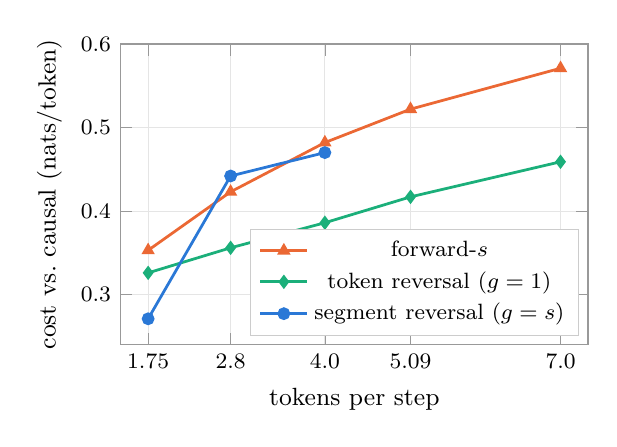
\begin{tikzpicture}
\begin{axis}[width=0.62\textwidth, height=5.4cm, xmin=1.4, xmax=7.35, ymin=0.24, ymax=0.6,
  xtick={1.75,2.8,4,5.09,7}, xticklabels={1.75,2.8,4.0,5.09,7.0},
  xlabel={tokens per step}, ylabel={cost vs.\ causal (nats/token)},
  grid=major, grid style={black!10}, axis line style={black!40}, tick style={black!40},
  label style={font=\small}, tick label style={font=\footnotesize},
  every axis plot/.append style={line width=1pt, mark size=1.8pt},
  legend style={font=\footnotesize, draw=black!20, at={(0.98,0.03)}, anchor=south east}]
\addplot[color=cOrange, mark=triangle*] coordinates {(1.75,0.353) (2.8,0.423) (4.0,0.482) (5.09,0.522) (7.0,0.571)};
\addlegendentry{forward-$s$}
\addplot[color=cAqua, mark=diamond*] coordinates {(1.75,0.326) (2.8,0.356) (4.0,0.386) (5.09,0.417) (7.0,0.459)};
\addlegendentry{token reversal ($g=1$)}
\addplot[color=cBlue, mark=*] coordinates {(1.75,0.271) (2.8,0.442) (4.0,0.470)};
\addlegendentry{segment reversal ($g=s$)}
\end{axis}
\end{tikzpicture}

  \caption{Cost against speed (seed 42, base model, 5000 steps; values in Appendix~\ref{app:sweep}). \rev beats \fwd at every speed, and the gap widens with parallelism. Segment reversal with $g=s$ is \sfill at 1.75 tokens per step, where it is the best schedule, but falls behind once a block has more than one jump token.}
  \label{fig:tradeoff}
\end{figure}

Sweeping the stagger from $s=8$ down to $s=0$ confirms that the advantage holds across the speed range (Figure~\ref{fig:tradeoff}).
\fwd drops adjacent pairs at every stagger, and its cost rises steeply with parallelism, whereas \rev never drops a pair closer than a block and degrades more slowly, so the gap between the two widens as more blocks run in parallel.
Segment reversal pays off only with two segments: shorter segments add jump tokens, and with four segments per block it is worse even than \fwd.
The best schedules we tested therefore form a single front, \sfill at 1.75 tokens per step and \rev beyond it, although above 1.75 tokens per step the advantage is so far established in likelihood rather than in samples (\S\ref{sec:samples}).

% ---------------------------------------------------------------------------
\section{The price: one jump token per block}
\label{sec:price}

\begin{figure}[t]
  \centering
  % Generated by scripts/make_figures.py -- do not edit by hand.
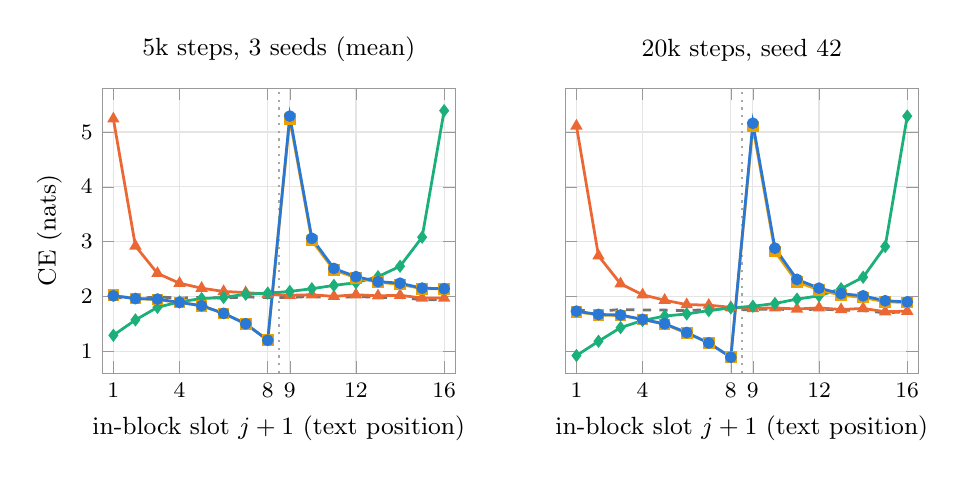
\begin{tikzpicture}
\begin{groupplot}[group style={group size=2 by 1, horizontal sep=1.4cm},
  width=0.5\textwidth, height=5.2cm, xmin=0.5, xmax=16.5, ymin=0.6, ymax=5.8,
  xtick={1,4,8,9,12,16}, ytick={1,2,3,4,5},
  xlabel={in-block slot $j+1$ (text position)}, ylabel={CE (nats)},
  grid=major, grid style={black!10}, axis line style={black!40},
  tick style={black!40}, label style={font=\small}, tick label style={font=\footnotesize},
  title style={font=\small}, every axis plot/.append style={line width=1pt, mark size=1.6pt},
  legend style={font=\footnotesize, draw=black!20,
    legend columns=5, /tikz/every even column/.append style={column sep=6pt}}]
\nextgroupplot[title={5k steps, 3 seeds (mean)}]
\draw[black!35, dotted, line width=0.8pt] (axis cs:8.5,0.6) -- (axis cs:8.5,5.8);
\addplot[color=black!55, mark=none, dashed] coordinates {(1,1.98) (2,1.96) (3,1.99) (4,1.97) (5,1.98) (6,1.97) (7,1.99) (8,1.98) (9,1.98) (10,2.00) (11,1.97) (12,2.00) (13,1.98) (14,1.98) (15,1.94) (16,1.94)};
\addplot[color=cOrange, mark=triangle*] coordinates {(1,5.24) (2,2.92) (3,2.42) (4,2.24) (5,2.15) (6,2.09) (7,2.07) (8,2.04) (9,2.02) (10,2.03) (11,2.00) (12,2.03) (13,2.01) (14,2.02) (15,1.97) (16,1.97)};
\addplot[color=cAqua, mark=diamond*] coordinates {(1,1.29) (2,1.57) (3,1.80) (4,1.90) (5,1.96) (6,1.98) (7,2.04) (8,2.06) (9,2.09) (10,2.14) (11,2.20) (12,2.25) (13,2.36) (14,2.55) (15,3.08) (16,5.39)};
\addplot[color=cYellow, mark=square*] coordinates {(1,2.02) (2,1.96) (3,1.94) (4,1.89) (5,1.83) (6,1.69) (7,1.50) (8,1.20) (9,5.24) (10,3.02) (11,2.48) (12,2.34) (13,2.26) (14,2.22) (15,2.14) (16,2.14)};
\addplot[color=cBlue, mark=*] coordinates {(1,2.01) (2,1.96) (3,1.95) (4,1.89) (5,1.83) (6,1.69) (7,1.50) (8,1.20) (9,5.29) (10,3.06) (11,2.51) (12,2.36) (13,2.27) (14,2.24) (15,2.15) (16,2.14)};
\nextgroupplot[title={20k steps, seed 42}, ylabel={}, yticklabels={}, legend to name=slotlegend]
\draw[black!35, dotted, line width=0.8pt] (axis cs:8.5,0.6) -- (axis cs:8.5,5.8);
\addplot[color=black!55, mark=none, dashed] coordinates {(1,1.75) (2,1.73) (3,1.76) (4,1.75) (5,1.75) (6,1.74) (7,1.76) (8,1.75) (9,1.76) (10,1.77) (11,1.75) (12,1.77) (13,1.75) (14,1.74) (15,1.70) (16,1.72)};
\addlegendentry{causal}
\addplot[color=cOrange, mark=triangle*] coordinates {(1,5.11) (2,2.74) (3,2.23) (4,2.03) (5,1.93) (6,1.85) (7,1.84) (8,1.80) (9,1.78) (10,1.79) (11,1.77) (12,1.79) (13,1.76) (14,1.78) (15,1.72) (16,1.73)};
\addlegendentry{forward-8}
\addplot[color=cAqua, mark=diamond*] coordinates {(1,0.92) (2,1.18) (3,1.43) (4,1.56) (5,1.64) (6,1.68) (7,1.74) (8,1.79) (9,1.82) (10,1.87) (11,1.95) (12,2.01) (13,2.14) (14,2.35) (15,2.91) (16,5.29)};
\addlegendentry{reverse-16}
\addplot[color=cYellow, mark=square*] coordinates {(1,1.72) (2,1.66) (3,1.65) (4,1.58) (5,1.49) (6,1.33) (7,1.15) (8,0.89) (9,5.10) (10,2.82) (11,2.26) (12,2.12) (13,2.02) (14,1.98) (15,1.90) (16,1.89)};
\addlegendentry{reverse-16-g8}
\addplot[color=cBlue, mark=*] coordinates {(1,1.73) (2,1.67) (3,1.66) (4,1.58) (5,1.50) (6,1.34) (7,1.15) (8,0.89) (9,5.16) (10,2.88) (11,2.31) (12,2.15) (13,2.05) (14,2.01) (15,1.92) (16,1.90)};
\addlegendentry{reverse-8-g8}
\end{groupplot}
\end{tikzpicture}

\par\smallskip\ref{slotlegend}

  \caption{Steady-state CE per in-block slot, in text order (slot 1 is the seam token). Left: 5000 steps, mean of seeds 42--44. Right: 20000 steps, seed 42. The dotted line separates the two halves of a block: \sfill writes slots 9--16 first and fills in slots 1--8 one stagger later. \fwd pays at the seam, \rev (shown in its order-only version) at the last slot, which it writes first, and \sfill at slot 9, its jump token, while its infilled left half falls below \causal. The \sfill curves with and without staggering nearly coincide, so almost none of its cost comes from dropped pairs. Values in Appendix~\ref{app:slots}.}
  \label{fig:slots}
\end{figure}

\paragraph{The cost moves from the seam to the jump token.}
Figure~\ref{fig:slots} shows where each schedule pays.
\fwd stays close to the causal model everywhere except at the seam, where the token's cross-entropy is more than two and a half times the causal value.
The reversed schedules show no seam spike, because the seam token is written with the previous block's tail in view.
Their cost appears instead at the token that is written first and predicted furthest ahead, which is the block's tail under \rev and the jump token under \sfill.
The left half that \sfill fills in afterwards even falls below the causal model, since each of its tokens is written with both neighbours known.

\paragraph{The terms do not cancel.}
If the model learned every conditional exactly, the jump token's loss and the infilled half's gain would cancel (Remark~\ref{rem:chain}).
They do not: even after four times longer training, the infilled half recovers only about two fifths of what the right half loses (Appendix~\ref{app:scaling}).
Predicting a token far ahead and infilling between two fixed contexts are harder conditionals to learn than next-token prediction, which is consistent with evidence that masked diffusion models, having to learn many orders, train on harder subproblems than left-to-right models~\citep{kim2025trainworst}.

\begin{table}[t]
  \centering
  \caption{Attempts to remove the ordering cost (seed 42). Each row trains the order-only version of \sfill, which drops nothing, so its entire cost over \causal in the same setting is ordering cost. The jump-token CE is the steady-state CE at slot 9, where \causal has 1.5--2.0 nats. $^\ast$\,Bound including the plan's negative log-likelihood, relative to \causal with the same plan; the token CE alone gives 0.191. Details in Appendices~\ref{app:scaling} and~\ref{app:remedies}.}
  \label{tab:attempts}
  \small
  \begin{tabular}{lrrrrr}
    \toprule
    Intervention & Params & Tokens & Steps & Ordering cost & Jump-token CE \\
    \midrule
    None (reference)                        & 7.2M  & 22M  & 5k  & 0.256 & 5.24 \\
    Longer training                         & 7.2M  & 22M  & 20k & 0.226 & 5.10 \\
    More parameters and data                & 31.5M & 219M & 20k & 0.242 & 4.95 \\
    Causal-mask mixing ($p=0.5$)            & 7.2M  & 22M  & 5k  & 0.338 & 5.32 \\
    Discrete block plan ($4\times16$ codes) & 7.2M  & 22M  & 5k  & 0.279$^\ast$ & 2.68 \\
    \bottomrule
  \end{tabular}
\end{table}

\paragraph{Nothing we tried removes the ordering cost.}
Table~\ref{tab:attempts} collects our attempts.
Training four times longer barely moves the ordering cost, and neither does a model with 4.4 times more parameters trained on ten times more data, which argues against the cost being a symptom of under-training or limited capacity, at least at this scale.
Mixing causal-mask steps into training makes it worse, mostly on the infilled half, so infilling is not a skill that ordinary left-to-right training supplies.
A discrete block-level plan helps where the guess ahead is largest: it lowers the ordering cost of \rev and roughly halves the cross-entropy of the \sfill jump token, but for \sfill the saving reappears as a plan that is harder to predict.
Finally, re-decoding the jump token once its block is written improves that token in samples but breaks the next one, which was written for the old value, so the break merely moves one position to the right (Appendix~\ref{app:refine}).

% ---------------------------------------------------------------------------
\section{In samples, a one-sided break is far milder than a seam}
\label{sec:samples}

Likelihood scores each token against real text, whereas samples test what a model writes when every token is its own.
For 512 development prompts we sample continuations at temperature $T=1$, each schedule in its own order and with all tokens of a serial step sampled in parallel.
An independently trained causal model judges them, since a model judging its own samples would only measure its own entropy.

\begin{table}[t]
  \centering
  \caption{Sample quality (seed-42 models, 5000 steps) under an independently trained causal judge. Judge CE is over the whole continuation; the seam is the first slot of steady-state blocks. Lower means more natural under the judge. $^\dagger$\,Non-causal.}
  \label{tab:samples}
  \small
  \begin{tabular}{lcrr}
    \toprule
    Source & Tokens/step & Judge CE & Judge CE at seam \\
    \midrule
    Real text            & $-$  & 2.02 & 2.04 \\
    \causal              & 1.00 & 2.61 & 2.56 \\
    \midrule
    \sfill               & 1.75 & \textbf{3.26} & \textbf{2.89} \\
    \rev                 & 1.75 & 3.56 & 7.12 \\
    \fwd                 & 1.75 & 3.47 & 11.29 \\
    \delayed             & 1.75 & 3.79 & 11.43 \\
    \midrule
    \landing$^\dagger$   & 7.00 & 3.61 & 6.15 \\
    \rev                 & 7.00 & 3.74 & 7.69 \\
    \fwd                 & 7.00 & 3.83 & 11.53 \\
    \bottomrule
  \end{tabular}
\end{table}

\paragraph{\sfill removes the seam failure.}
Under \fwd the seam token is by far the least natural token in a sample: written blind to its left neighbour, it often fails to connect to it.
Under \sfill the judge scores the seam almost as it scores the same position in causal samples (2.9 against 2.6 nats; Table~\ref{tab:samples}), and \sfill samples are also more natural overall than those of \fwd at the same speed.
The same holds for models trained four times longer and for the wide model (Appendix~\ref{app:samples}).
\rev, by contrast, repairs the seam only partly, so at this parallelism \sfill is the variant to use.

\paragraph{A jump token is as hard to predict as a seam token, but breaks half as badly.}
In likelihood, the jump token of \sfill and the seam token of \fwd are about equally hard (Table~\ref{tab:main}), yet in samples the judge's cross-entropy at the jump token is half that at a forward or delayed seam.
The difference lies in what is written around them.
At a forward seam, the head of a block and the tail of the previous block are written blind to each other, so nothing reconciles them, whereas at a jump token the infilled half is written afterwards and conditions on it, so the junction is repaired from one side.
The tokens that the judge finds least plausible tell the same story.
Under \fwd more than a third of them fall on the seam, six times the share of a uniform spread, while under \sfill the largest share falls on the jump token and is half as large (Appendix~\ref{app:examples}, which also shows unselected samples).

\paragraph{Read-ahead works for the same reason.}
At full parallelism the non-causal \landing produces more natural samples than \rev, although its likelihood is worse, because it too joins each seam from one side: the next block's head is written first, and the whole block before it then runs towards that head.
\rev also writes each head after the previous tail, but leaves a single token to join two sides that are already fixed.
The price of reading ahead is that a block cannot be finished before the head of the next block is sampled, so a streaming decoder must keep one block of lookahead, whose heads are written blind, and can no longer commit each block from the past alone.
Since reordering and reading ahead are orthogonal, the two could be combined.

% ---------------------------------------------------------------------------
\section{Related work}
\label{sec:related}

\paragraph{Staggered and parallel generation.}
Starting the next unit before the current one is finished is an old idea, from wavefront parallel processing in HEVC~\citep{sullivan2012hevc} to row-staggered and region-parallel image generation~\citep{he2025zipar,wang2025par}, diagonal video decoding~\citep{ye2025diagonal}, MusicGen's codebook delays~\citep{copet2023musicgen}, depth staggering~\citep{cutler2025stagformer} and concurrent generators over a shared cache~\citep{rodionov2025hogwild}.
In text, LCLM interleaves staggered lines~\citep{li2026lclm}, LatLM locates the cost at each line's first token and mitigates it by waiting or deferring commitment~\citep{zhang2026latlm}, and Predictive-State Flows repairs block boundaries with non-causal landing targets~\citep{he2026psf}.
Block diffusion pipelines overlap blocks and repair seams by refinement, temporary context or verification~\citep{arriola2025block,tsou2026tecop,tian2026flowblock,jin2026multibd,ren2026asynclane,chavan2026lafa}.
All of these write tokens left to right within a unit; Table~\ref{tab:remedies} contrasts their remedies, and Appendix~\ref{app:related} compares the closest work in detail.

\paragraph{Generation order.}
That dependency decays with distance has motivated parallel decoding of distant regions~\citep{wang2025par,he2025zipar} and serialising adjacent tokens~\citep{li2025refusion}, and total correlation explains parallel-decoding error~\citep{zhang2026generation}.
Order also matters for learning, even though the chain rule holds for any order.
Reversing the source sentence eased LSTM sequence-to-sequence learning by bringing dependent words close together~\citep{sutskever2014seq2seq}, the order of inputs and outputs changes what a model learns~\citep{vinyals2016order}, any-order autoregressive models improve when trained on fewer orders~\citep{shih2022aoarm}, masked diffusion models train on provably harder subproblems than left-to-right models~\citep{kim2025trainworst}, and block diffusion models prefer left-to-right unmasking~\citep{hou2026rethinking}.
Writing the seam last uses order the other way round: it accepts a harder order to keep the strongest dependency, and our decomposition measures the price of that order separately from the information it keeps.
Our measurement device is XLNet's two-stream attention~\citep{yang2019xlnet}.
Arbitrary-order generation~\citep{pannatier2024sigma}, fill-in-the-middle training~\citep{bavarian2022fim}, within-block right-to-left baselines~\citep{yao2026orderagnostic} and bidirectional generation towards the middle~\citep{zhou2019bothsides,zhou2019sbnmt,zhang2020interleaved,nguyen2023meet} are related orders, and our meet-in-the-middle baseline (Appendix~\ref{app:meet}) is a causal, block-level adaptation of the last.

\paragraph{Exact and approximate parallel decoding.}
Semi-autoregressive translation generates adjacent tokens at once~\citep{wang2018semi}, dropping exactly the dependencies that writing the seam last keeps, and non-autoregressive translation drops all of them~\citep{gu2018nat}.
Draft-and-verify methods keep the causal distribution, exactly or approximately: blockwise parallel decoding~\citep{stern2018blockwise}, speculative decoding~\citep{leviathan2023speculative,chen2023speculative}, EAGLE~\citep{li2024eagle}, lookahead decoding~\citep{fu2024lookahead} and multi-token prediction~\citep{gloeckle2024mtp}.
Writing the seam last targets decoders that commit tokens without verification.

% ---------------------------------------------------------------------------
\section{Limitations}
\label{sec:limitations}

\begin{itemize}
  \item \textbf{Scale and seeds.} The study uses TinyStories and models of 7.2M--31.5M parameters. The main comparison uses three seeds; most ablations use one, including the stagger sweep, meet-in-the-middle, scaling, plans, refinement and the samples. Whether much larger models remove the ordering cost remains open.
  \item \textbf{The ordering cost remains.} Writing the seam last pays about 0.23--0.27 nats/token relative to a causal model, and about 0.65--0.8 judge nats in samples, in every setting we sampled. Our tests of plans, refinement and causal-mask mixing are narrow and do not rule out other remedies.
  \item \textbf{High parallelism.} The advantage of \rev above 1.75 tokens per step is shown in likelihood, not in samples. We ran no temperature sweep and no comparison with LatLM-style waiting.
  \item \textbf{Practicality.} Reversed order emits text a block at a time, which delays the first readable token. The schedules need training, and tokens per step is not wall-clock speed.
\end{itemize}

% ---------------------------------------------------------------------------
\section{Conclusion}

A parallel decoder cannot keep every dependency, but it can choose which ones to give up, and staggered pipelines that write each block left to right give up the worst one, the seam.
Writing the seam last keeps the parallelism, stays causal and moves every dropped dependency at least a block away; with the number of dropped pairs fixed, that move alone makes them more than twenty times cheaper and removes the seam failure from samples.
What remains is an ordering cost at one jump token per block, which the tokens written around it only partly repair.
For designers of block-parallel decoders, the lesson is to choose the write order so that the dependencies a schedule must drop are the distant ones, and to measure the ordering cost separately, because it reflects learnability rather than information and is the cost that larger models, continuous block latents or read-ahead would have to remove.

% ---------------------------------------------------------------------------
\subsection*{AI use statement}
Apart from the four parts listed next, this work is the author's own, including the research question, the central idea of writing each block's head after the previous block's tail, and the design of the study, such as the meet-in-the-middle baseline and the scaling experiment.
The author used an AI assistant (Claude) to design the concrete schedules that implement the central idea (\rev, \sfill and segment reversal in general), to derive the proofs of their distance bounds, to write the code and run the experiments, and to draft most of the text.
The author directed this work and checked all results, and the distance bounds are additionally verified by exhaustive tests (Appendix~\ref{app:proofs}).
The author takes full responsibility for the content of this paper, including text, claims and artifacts produced with the aid of generative AI.

\subsection*{Reproducibility statement}
The schedules, the two-stream and plan-conditioned models, the sample evaluation and the exhaustive tests of Propositions~\ref{prop:general} and~\ref{prop:meet} are implemented in a single code base.
Appendix~\ref{app:details} lists the architecture, data, optimiser and evaluation protocol, and Appendix~\ref{app:proofs} the verified properties.

\bibliography{refs}
\bibliographystyle{iclr2027_conference}

\appendix

% ---------------------------------------------------------------------------
\section{Proofs and exhaustive verification}
\label{app:proofs}

Proposition~\ref{prop:distance} is a special case of the following statement for any stagger and segment length.

\begin{proposition}[Dropped pairs of $\Rsg{s}{g}$]
\label{prop:general}
Let $g\mid L$ and $B\ge2$.
(a) If $s\ge L$, $\Rsg{s}{g}$ drops no pair.
(b) If $0\le s\le L-1$, every pair that $\Rsg{s}{g}$ drops has distance at least
\begin{equation}
  \dmin(L,s,g) \;=\; L-g+1+g\cdot\pos{\left\lceil \tfrac{s-g+1}{g}\right\rceil},
  \label{eq:dmin}
\end{equation}
and some dropped pair has distance exactly $\dmin$.
(c) If $0\le s\le L-1$, $\Fs{s}$ drops the pair $(t-1,L-1),(t,0)$ for every $t\ge1$, and it drops exactly as many pairs as $\Rsg{s}{1}$ and, if $s=L/2$, as $\Rsg{s}{s}$.
\end{proposition}

For $g=1$, \eqref{eq:dmin} gives $\dmin=L+s$, and for $s=g<L$ it gives $\dmin=L+1$, which is Proposition~\ref{prop:distance}(i) for \rev and \sfill; part~(c) is Proposition~\ref{prop:distance}(ii).

\begin{proof}
Write $Q=L/g$ and, for slot $j$, $q=\lfloor j/g\rfloor\in\{0,\dots,Q-1\}$ and $r=j\bmod g\in\{0,\dots,g-1\}$.

\emph{Pairs inside one block are never dropped.}
For fixed $t$, the map $j\mapsto(Q-1-q)g+r$ is a bijection from $\{0,\dots,L-1\}$ onto itself.
Two distinct tokens of the same block therefore have distinct clocks, and by~\eqref{eq:visibility} the later one reads the earlier one.
The same holds for $\Fs{s}$.

\emph{Condition for a cross-block pair to be dropped.}
Let $a=(t',j')$ and $b=(t,j)$ with $t'<t$, and let $m=t-t'\ge1$.
Token $a$ never reads $b$, because $b$ lies in a block to its right.
So the pair is dropped if and only if $b$ does not read $a$, that is, $\tau(a)\ge\tau(b)$.
Let $k=q-q'$ and $\delta=r-r'\in\{-(g-1),\dots,g-1\}$.
By~\eqref{eq:clock}, $\tau(a)-\tau(b)=-sm+kg-\delta$, so
\begin{equation}
  \text{$(a,b)$ is dropped} \iff kg-\delta\ \ge\ sm,
  \label{eq:dropcond}
\end{equation}
and its distance is $(P+tL+j)-(P+t'L+j') = mL+kg+\delta$.

\emph{(a).}
Since $k\le Q-1$ and $-\delta\le g-1$, we have $kg-\delta\le (Q-1)g+g-1=L-1$.
If $s\ge L$, then $sm\ge L>L-1$, so~\eqref{eq:dropcond} never holds.

\emph{(b), lower bound.}
Assume $0\le s\le L-1$ and let $(a,b)$ be dropped.
First, $k\ge0$: by~\eqref{eq:dropcond}, $kg\ge sm+\delta\ge-(g-1)>-g$.
Let $k^\ast=\pos{\lceil (s-g+1)/g\rceil}$.
Then $k^\ast\le Q-1$: this is trivial if $k^\ast=0$, and otherwise $(s-g+1)/g\le (L-g)/g=Q-1$, which is an integer.
If $m=1$, then by~\eqref{eq:dropcond} $kg\ge s+\delta\ge s-g+1$, so $k\ge\lceil (s-g+1)/g\rceil$, and together with $k\ge0$ we get $k\ge k^\ast$.
Hence the distance is $L+kg+\delta\ \ge\ L+k^\ast g-(g-1)=\dmin$.
If $m\ge2$, then using $k\ge0$ and $\delta\ge-(g-1)$, the distance is at least $2L-g+1$.
Because $k^\ast\le Q-1$, we have $\dmin\le L-g+1+(L-g)=2L-2g+1<2L-g+1$, so every such pair is strictly farther apart than $\dmin$.

\emph{(b), tightness.}
Take $t'=0$, $t=1$, $q'=0$, $q=k^\ast$, $r'=g-1$ and $r=0$, which is valid because $k^\ast\le Q-1$.
Then $kg-\delta=k^\ast g+g-1\ge s$, since $k^\ast g\ge s-g+1$, so the pair is dropped, and its distance is $L+k^\ast g-(g-1)=\dmin$.

\emph{(c).}
Under $\Fs{s}$, $\tau(t-1,L-1)=s(t-1)+L-1\ge st=\tau(t,0)$, so $(t,0)$ cannot read $(t-1,L-1)$, which never reads a block to its right.
For blocks $t-m$ and $t$, $\Fs{s}$ drops $(t-m,j'),(t,j)$ if and only if $j'-j\ge sm$, and $\Rsg{s}{1}$ if and only if $j-j'\ge sm$ (by~\eqref{eq:dropcond} with $g=1$); the reflection $(j,j')\mapsto(L-1-j,\,L-1-j')$ maps one set onto the other.
Now let $s=g=L/2$, so that $Q=2$.
For adjacent blocks, \eqref{eq:dropcond} reads $kg-\delta\ge g$; since $k\in\{0,1\}$ for a dropped pair and $-\delta\le g-1$, this forces $k=1$, that is $q'=0$ and $q=1$, and $\delta\le0$, that is $r\le r'$, which gives $g(g+1)/2$ pairs.
Blocks $m\ge2$ apart would need $kg-\delta\ge 2g=L$, which is impossible.
Under $\Fs{s}$, adjacent blocks drop the pairs with $j'-j\ge s$, of which there are $\sum_{d=s}^{L-1}(L-d)=(L-s)(L-s+1)/2=g(g+1)/2$, and blocks $m\ge2$ apart would need $j'-j\ge 2s=L$.
Both schedules therefore drop $g(g+1)/2$ pairs between each pair of adjacent blocks and none otherwise.
\end{proof}

\paragraph{Exhaustive verification.}
For every $L\in\{8,16\}$, every segment length $g\in\{1,2,4,8\}$ with $g\mid L$, and every stagger $s=0,\dots,L$, we built the visibility matrix of $\Rsg{s}{g}$ for a 3-token prompt and $B=5$ blocks, enumerated all dropped pairs, and checked that their minimum distance equals~\eqref{eq:dmin} whenever any pair is dropped.
For the meet-in-the-middle schedule \meet{d} (Appendix~\ref{app:meet}), we checked against an independent simulation of the write order that the reversed block's head reads the forward block's tail, and that the minimum dropped distance is $d+1$.
The test suite also checks that every schedule's visibility relation is transitive and acyclic; that forward staggering drops adjacent pairs while reversed staggering drops only distant ones; that the seam token of \rev sees the previous block's tail; that under \rev with $s=0$ slot $j$ sees exactly the slots $j'>j$ of the previous block; that \landing tokens read only the next block's first token; that two-stream predictions are invariant to the content of invisible tokens; and that the sampler's number of serial rounds matches each schedule's parallelism.

% ---------------------------------------------------------------------------
\section{Experimental details}
\label{app:details}

\paragraph{Models.}
Both models are two-stream Transformers with SwiGLU feed-forward layers, RMSNorm, learned positions and tied embeddings.
The base model has width 256, 6 layers, 4 heads and feed-forward width 768 (7.2M parameters); the wide model has width 512, 8 layers, 8 heads and feed-forward width 1536 (31.5M parameters).

\paragraph{Data.}
We train on 100k TinyStories~\citep{eldan2023tinystories} stories (22.0M tokens) with an 8192-token vocabulary, and evaluate on a disjoint development split of 10{,}995 stories.
Windows are drawn at random from the concatenated, EOS-separated stream; each has a 16-token prompt followed by $B=7$ blocks of $L=16$.
The 219M-token run of Appendix~\ref{app:scaling} uses 1M stories with the same tokenizer and the same development split.

\paragraph{Optimisation.}
All arms use AdamW ($\beta=(0.9,0.95)$, weight decay 0.1), a peak learning rate of $10^{-3}$ with 200 warm-up steps and cosine decay to $0.1\times$, gradient clipping at 1.0, batch size 64 and bf16 autocast, for 5000 steps unless stated otherwise.

\paragraph{Evaluation.}
CE is measured on 4096 fixed development windows and restricted to steady-state blocks $t\ge2$, because blocks 0 and 1 still read the prompt as their predecessor.
Samples use 512 development prompts, temperature $T=1$ and the same sampling seed for every schedule; the judge is a causal model trained with a different seed (or, in Appendix~\ref{app:samples}, at a different size or length), so that judge and judged are always trained independently.

\paragraph{Per-slot cross-entropy.}
\label{app:slots}
Table~\ref{tab:slots} gives the values plotted in Figure~\ref{fig:slots} (left).

\begin{table}[h]
  \centering
  \caption{Steady-state CE per in-block slot (text order; slot 1 is the seam), 5000 steps, mean of seeds 42--44. ``Order only'' is the same write order without staggering.}
  \label{tab:slots}
  \scriptsize
  \setlength{\tabcolsep}{2.0pt}
  \begin{tabular}{l*{16}{r}}
    \toprule
    Slot & 1 & 2 & 3 & 4 & 5 & 6 & 7 & 8 & 9 & 10 & 11 & 12 & 13 & 14 & 15 & 16 \\
    \midrule
    \causal               & 1.98 & 1.96 & 1.99 & 1.97 & 1.98 & 1.97 & 1.99 & 1.98 & 1.98 & 2.00 & 1.97 & 2.00 & 1.98 & 1.98 & 1.94 & 1.94 \\
    \fwd                  & 5.24 & 2.92 & 2.42 & 2.24 & 2.15 & 2.09 & 2.07 & 2.04 & 2.02 & 2.03 & 2.00 & 2.03 & 2.01 & 2.02 & 1.97 & 1.97 \\
    \rev, order only      & 1.29 & 1.57 & 1.80 & 1.90 & 1.96 & 1.98 & 2.04 & 2.06 & 2.09 & 2.14 & 2.20 & 2.25 & 2.36 & 2.55 & 3.08 & 5.39 \\
    \sfill, order only    & 2.02 & 1.96 & 1.94 & 1.89 & 1.83 & 1.69 & 1.50 & 1.20 & 5.24 & 3.02 & 2.48 & 2.34 & 2.26 & 2.22 & 2.14 & 2.14 \\
    \sfill                & 2.01 & 1.96 & 1.95 & 1.89 & 1.83 & 1.69 & 1.50 & 1.20 & 5.29 & 3.06 & 2.51 & 2.36 & 2.27 & 2.24 & 2.15 & 2.14 \\
    \bottomrule
  \end{tabular}
\end{table}

% ---------------------------------------------------------------------------
\section{Further schedules}
\label{app:schedules}

\subsection{Segment length and the stagger sweep}
\label{app:sweep}

\begin{table}[t]
  \centering
  \caption{Effect of the segment length $g$ (seed 42, 5000 steps; steady-state CE, \causal 1.977). $g=1$ is \rev and $g=8$ is \sfill. Information cost = staggered $-$ order-only CE; ordering cost = order-only cost vs.\ \causal.}
  \label{tab:segment}
  \small
  \begin{tabular}{crrrr}
    \toprule
    $g$ & Order only, $\Rsg{16}{g}$ & Staggered, $\Rsg{8}{g}$ & Information cost & Ordering cost \\
    \midrule
    1 & 2.294 & 2.304 & 0.010 & 0.316 \\
    4 & 2.386 & 2.401 & 0.015 & 0.409 \\
    \textbf{8} & \textbf{2.234} & \textbf{2.248} & 0.015 & \textbf{0.256} \\
    \bottomrule
  \end{tabular}
\end{table}

\begin{table}[t]
  \centering
  \caption{Cost vs.\ \causal (nats/token) across the stagger $s$ (seed 42, base model, 5000 steps), with the distance of the closest dropped pair in parentheses. Tokens per step are measured over the seven blocks of a window; in the steady state they approach $L/s$. For $s=1$, segment reversal with $g=s$ is \rev.}
  \label{tab:tradeoff}
  \small
  \begin{tabular}{crrrr}
    \toprule
    Tokens/step & $s$ & \fwd, $\Fs{s}$ & \rev, $\Rsg{s}{1}$ & Segment, $\Rsg{s}{s}$ \\
    \midrule
    1.75 & 8 & 0.353 (1) & 0.326 (24) & \textbf{0.271} (17) \\
    2.80 & 4 & 0.423 (1) & \textbf{0.356} (20) & 0.442 (17) \\
    4.00 & 2 & 0.482 (1) & \textbf{0.386} (18) & 0.470 (17) \\
    5.09 & 1 & 0.522 (1) & \textbf{0.417} (17) & $-$ \\
    7.00 & 0 & 0.571 (1) & \textbf{0.459} (16) & $-$ \\
    \bottomrule
  \end{tabular}
\end{table}

\paragraph{The ordering cost depends on the segment length.}
Varying the segment length at a fixed stagger (Table~\ref{tab:segment}) leaves the information cost small for every $g$, while the ordering cost is non-monotonic in $g$, lowest for the two-segment \sfill and highest for $g=4$.
The per-slot CE points to backward jumps, each of which starts a segment whose first token is predicted far ahead of the visible text: the three jump tokens of a block under $\Rsg{16}{4}$ cost 4.11, 4.46 and 5.34 nats, whereas \sfill has a single jump (5.24).
\rev also has a single far-ahead token, the tail, but writes the whole block against the natural direction.
Segment reversal does not help at $s=0$ either: $\Rsg{0}{4}$ costs 0.561, consistent with its smaller $\dmin=13$.

\paragraph{The stagger sweep.}
Table~\ref{tab:tradeoff} gives the values of Figure~\ref{fig:tradeoff}.
The margin of \rev over \fwd grows from 0.027 at 1.75 tokens per step to 0.112 at 7.00, and taking the best reversed schedule at each speed, from 0.082 to 0.112.
Shorter segments add backward jumps, three per block for $g=4$ and seven for $g=2$: under $\Rsg{4}{4}$ the three jump tokens cost 4.13, 4.52 and 5.47 nats, against about 1.98 for \causal, which makes the schedule worse than $\Fs{4}$, and $\Rsg{2}{2}$ is only slightly better than $\Fs{2}$ and far behind \rev.
\rev makes one jump per block, writing the tail first; its per-slot CE is a smooth ramp, from 1.34 at the head to 5.58 at the tail for $s=2$, and its cost grows slowly with parallelism.
These are single-seed likelihood results for the base model.

\subsection{Meet-in-the-middle}
\label{app:meet}

We adapt generation from both sides towards the middle to blocks with two schedules.
Under \meet{d}, blocks are decoded in pairs, one pair after another: block $2p$ runs forward and block $2p+1$ runs in reverse, starting $d$ steps later,
\begin{equation}
  \tau(2p,j)=p(L+d)+j,\qquad \tau(2p+1,j)=p(L+d)+d+(L-1-j).
  \label{eq:meet}
\end{equation}
The two blocks meet at their common seam, and the reversed block's head is written last.
Under \alt{d}, every block starts $d$ steps after its predecessor and directions alternate: $\tau(t,j)=td+j$ for even $t$ and $td+L-1-j$ for odd $t$.
Unlike sentence-level bidirectional decoders~\citep{zhou2019sbnmt,zhang2020interleaved}, \meet{d} does not let the forward block read its reversed partner, which lies to its right.
\meet{d} needs $\lfloor B/2\rfloor(L+d)+(B\bmod 2)L$ steps, which gives 1.67 tokens per step for $d=1$ and 1.47 for $d=4$; \alt{d} needs $(B-1)d+L$, which gives 5.09 for $d=1$.

\begin{proposition}[Meet-in-the-middle]
\label{prop:meet}
Under \meet{d} or \alt{d} with $0\le d\le L-1$ and $B\ge2$, every dropped pair has distance at least $d+1$, and some dropped pair has distance exactly $d+1$.
\end{proposition}

\begin{proof}
Inside a block the clock is a bijection onto $L$ consecutive steps, so no pair inside a block is dropped.
Let $a=(t-1,j')$ and $b=(t,j)$.
First let block $t-1$ run forward and block $t$ in reverse: the two blocks of a \meet{d} pair, or an even $t-1$ under \alt{d}.
Under both schedules $\tau(a)-\tau(b)=j+j'-(L-1)-d$, so the pair is dropped if and only if $j+j'\ge L-1+d$.
Its distance is $L+j-j'=L+(j+j')-2j'\ge L+(L-1+d)-2(L-1)=d+1$, with equality at $j'=L-1$ and $j=d$.
Under \alt{d}, if block $t-1$ runs in reverse and block $t$ forward, then $\tau(a)-\tau(b)=L-1-d-j-j'$; the pair is dropped if and only if $j+j'\le L-1-d$, and its distance is $L+j-j'\ge L-j'\ge d+1$.
Under \meet{d}, every token of pair $p+1$ is written after all tokens of pair $p$, so no pair across groups is dropped.
Under \alt{d}, tokens in blocks $m\ge2$ apart are at least $mL-(L-1)\ge L+1>d+1$ apart.
\end{proof}

\begin{table}[t]
  \centering
  \caption{Meet-in-the-middle against reversed staggering (seed 42, 5000 steps; cost vs.\ \causal of the same seed, so values differ slightly from the 3-seed means in Table~\ref{tab:main}). Dropped pairs are counted per window. Per-direction costs are averages over forward and reversed blocks.}
  \label{tab:meet}
  \small
  \begin{tabular}{lcrrrrr}
    \toprule
    Schedule & \makecell{Tokens\\per step} & \makecell{Closest\\pair} & \makecell{Dropped\\pairs} & \makecell{$\Delta$ vs.\\causal} & \makecell{Forward\\blocks} & \makecell{Reversed\\blocks} \\
    \midrule
    \sfill          & 1.75 & 17 & 216  & \textbf{0.271} & $-$ & $-$ \\
    \meet{4}        & 1.47 & 5  & 234  & 0.285 & $\approx0.13$ & $\approx0.51$ \\
    \meet{1}        & 1.67 & 2  & 360  & 0.318 & $\approx0.14$ & $\approx0.58$ \\
    \fwd            & 1.75 & 1  & 216  & 0.353 & $-$ & $-$ \\
    \midrule
    \rev            & 7.00 & 16 & 2856 & \textbf{0.459} & $-$ & $-$ \\
    \alt{1}         & 5.09 & 2  & 2030 & 0.466 & $\approx0.36$ & $\approx0.62$ \\
    \bottomrule
  \end{tabular}
\end{table}

At similar parallelism, meet-in-the-middle drops both more pairs and closer ones (Table~\ref{tab:meet}), and reversed staggering is better on both axes: \sfill is more parallel than \meet{4} and \meet{1} and cheaper than both, and at high parallelism \rev matches \alt{1} in cost at higher parallelism.
Meet-in-the-middle does remove the seam failure, but almost all of its cost sits on the reversed blocks.
The first token a reversed block writes is its tail, and at that moment its forward partner has written only $d$ tokens, so the tail has no written neighbours nearby and must be guessed about a block ahead.
The smaller cost of about 0.13 on the forward blocks is plausibly the price of one model learning both directions.

\subsection{Reading every schedule by which pairs it drops}
\label{sec:lens}

The same lens accounts for every schedule we tested (Tables~\ref{tab:main} and~\ref{tab:meet}; pair counts per window from the visibility masks).
\begin{itemize}
  \item At $s=8$, \fwd, \rev and \sfill drop the same 216 pairs, at distance 1--8, 24 or more, and 17 or more, and their information costs are 0.350, 0.016 and 0.012.
  \item At $s=0$, \fwd and \rev drop 2856 pairs each. The cost is 0.570 when the closest dropped pair is adjacent and 0.466 when it is 16 tokens apart.
  \item \delayed drops all 1536 pairs between adjacent blocks, including the adjacent ones, and costs 0.508.
  \item \landing keeps the tail, because every token after a block's head reads the next block's head, but it blinds the head, which is written at step~0 with only the prompt in view. Its first-token CE is 5.83, against 1.46 for its last token.
  \item \meet{1} drops more pairs than reversed staggering (360), some of them near (distance 2), and costs 0.318. With a longer lag, \meet{4} drops 234 pairs, none closer than 5, and costs 0.285.
\end{itemize}
This is a qualitative reading of a handful of schedules at one small scale, not a fitted law.
Where the count is fixed, a larger closest distance means a lower cost; across schedules, the ranking follows the pair count and the closest distance together.

% ---------------------------------------------------------------------------
\section{Scaling}
\label{app:scaling}

\begin{table}[t]
  \centering
  \caption{Cost vs.\ \causal at checkpoints of a single 20000-step run (seed 42, base model). Intermediate checkpoints lie in the high-learning-rate part of a 20000-step cosine schedule and are not directly comparable to separate 5000-step runs.}
  \label{tab:long}
  \small
  \begin{tabular}{rrrrrrr}
    \toprule
    Step & \makecell{\causal\\CE} & \makecell{\rev,\\order only} & \makecell{\sfill,\\order only} & \sfill & \fwd & \makecell{\fwd $-$\\\sfill} \\
    \midrule
    5k  & 2.041 & 0.299 & 0.247 & 0.265 & 0.350 & 0.085 \\
    10k & 1.881 & 0.289 & 0.245 & 0.262 & 0.356 & 0.094 \\
    15k & 1.788 & 0.280 & 0.233 & 0.252 & 0.359 & 0.106 \\
    20k & 1.748 & 0.270 & 0.226 & 0.246 & 0.355 & 0.109 \\
    \bottomrule
  \end{tabular}
\end{table}

\begin{table}[t]
  \centering
  \caption{Capacity at 5000 steps (seed 42). Cost vs.\ \causal of the same size; the last column is the base model at 20000 steps for comparison.}
  \label{tab:wide}
  \small
  \begin{tabular}{lrrr}
    \toprule
     & Base (7.2M) & Wide (31.5M) & Base, 20k steps \\
    \midrule
    \causal CE                              & 1.977 & 1.772 & 1.748 \\
    \sfill, order only (ordering cost)      & 0.256 & 0.272 & 0.226 \\
    \sfill                                  & 0.271 & 0.296 & 0.246 \\
    \fwd                                    & 0.353 & 0.389 & 0.355 \\
    \fwd $-$ \sfill                         & 0.083 & 0.093 & 0.109 \\
    \bottomrule
  \end{tabular}
\end{table}

\begin{table}[t]
  \centering
  \caption{Ordering cost (order-only \sfill $-$ \causal, steady-state CE, nats/token) at checkpoints of single 20000-step runs (seed 42). Only these two schedules were trained at the wide size for 20000 steps.}
  \label{tab:widelong}
  \small
  \begin{tabular}{rrrrrrr}
    \toprule
    & \multicolumn{2}{c}{Base, 22M tokens} & \multicolumn{2}{c}{Wide, 22M tokens (overfits)} & \multicolumn{2}{c}{Wide, 219M tokens} \\
    \cmidrule(lr){2-3}\cmidrule(lr){4-5}\cmidrule(lr){6-7}
    Step & Causal CE & Ordering cost & Causal CE & Ordering cost & Causal CE & Ordering cost \\
    \midrule
    5k  & 2.041 & 0.247 & 1.878 & 0.265 & 1.855 & 0.277 \\
    10k & 1.881 & 0.245 & 1.730 & 0.234 & 1.685 & 0.257 \\
    15k & 1.788 & 0.233 & 1.659 & 0.190 & 1.566 & 0.248 \\
    20k & 1.748 & 0.226 & 1.652 & 0.146 & 1.508 & \textbf{0.242} \\
    \bottomrule
  \end{tabular}
\end{table}

\paragraph{Training length.}
Over four times more training (Table~\ref{tab:long}), the cost of \fwd stays at about 0.35, because it is information loss, which training does not recover.
The ordering cost of \sfill shrinks only slowly, by about 9\% from 0.247 to 0.226, while causal CE falls by 0.29.
Because one cost is flat and the other decreases, the advantage of \sfill over \fwd grows from 0.085 to 0.109.

\paragraph{Capacity.}
With 4.4 times more parameters at 5000 steps (Table~\ref{tab:wide}), the ordering cost does not shrink (0.256 to 0.272), while the information cost of \fwd grows (0.353 to 0.389), plausibly because a stronger model exploits adjacent dependencies more and so loses more when they are cut.
The advantage of \sfill grows in this direction too (0.083 to 0.093), and its information cost stays small in every setting: 0.020 at 20k steps and 0.024 for the wide model.

\paragraph{Capacity with longer training needs more data.}
On the usual 22M-token training set, the wide model's ordering cost appears to fall from 0.265 to 0.146 over 20000 steps (Table~\ref{tab:widelong}), but the drop comes from an overfitting baseline.
The wide causal model sees that training set about 7.4 times and stops improving after 15k steps; at 20k steps its training loss is about 1.32 against a development CE of 1.705 over all blocks, while the order-only model overfits much less (about 1.69 against 1.85).
On 1M stories (219M tokens, less than one epoch in 20000 steps), training and development CE stay close (about 1.51 and 1.56), and the ordering cost is 0.242 at 20k steps, the same as the base model's.
It falls by only 0.035 while causal CE improves by 0.35, so relative to causal CE it rises slightly, from 15\% to 16\%.
The base model's 20k-step runs overfit mildly (causal training loss about 1.67 against 1.80 on development data), so its 0.226 is slightly optimistic.

\paragraph{Where the models pay.}
For the base model at 20k steps, summed over a block, the jump token costs $+3.34$ nats and the rest of the right half $+2.79$, while the infilled half gains only $-2.52$, a net cost of 0.226 nats per token.
The wide model at 20k steps on 219M tokens behaves in the same way.
Its causal CE is 1.47--1.53 per slot; the infilled head falls from 1.48 to 0.67 across its eight slots, all below causal; the jump token stays at 4.95 (5.19 at 5k steps); and the rest of the right half runs from 2.63 down to 1.68.
Summed over a block, the jump token costs $+3.44$ nats and the rest of the right half $+3.05$, while the infilled head gains $-2.62$, a net $+3.88$ nats per block, or 0.242 per token.
In both models the infilled half thus recovers only about two fifths of what the right half loses, although with exact conditionals the terms would cancel (Remark~\ref{rem:chain}).
Across 7.2M--31.5M parameters and up to 20000 steps, with enough data, our models do not approach that limit; this rests on one seed and on the order-only \sfill only.

% ---------------------------------------------------------------------------
\section{Attempts to remove the ordering cost}
\label{app:remedies}

\subsection{Mixing causal-mask training}
\label{app:mixing}

One might suspect that the ordering cost reflects a representation deficit that ordinary left-to-right training could fill.
We therefore trained the same model on the causal mask with probability $p$ at each step, and evaluated it under the target schedule (seed 42).
Costs got worse throughout: \sfill went from 0.271 at $p=0$ to 0.291 at $p=0.25$ and 0.351 at $p=0.5$, its order-only version from 0.256 to 0.338 at $p=0.5$, and \rev at $s=0$ from 0.459 to 0.658 at $p=0.5$.
The degradation sits mostly in the infilled left half: the last-written slot (slot 8) of \sfill rises from 1.19 to 1.63 at $p=0.5$, while the first-written right half is almost unchanged.
Infilling is a conditional that needs its own training signal.

\subsection{A discrete block-level plan}
\label{sec:latent}

The ordering cost is concentrated in conditionals that have to guess ahead: the first-written token of a block under \rev, the half-block jump under \sfill, and the tail of a reversed block under meet-in-the-middle.
A token-level model has no block-level plan to rely on in any of these cases.
In block-latent language models~\citep{shao2025calm,he2026psf,li2026lclm}, each block has a latent that encodes its content before any token is emitted.
Once the model knows roughly what the block says, it no longer has to guess the block's tail blind, so the order in which a block's tokens are written might matter much less.
We test this hypothesis with a deliberately simple discrete plan.

\paragraph{Plan-conditioned model.}
We extend the two-stream model with $K=4$ discrete plan codes per generated block, each taking one of $V=16$ values, so a plan carries at most $K\ln V\approx11.1$ nats per block.
An encoder, a one-hidden-layer MLP over the concatenated token embeddings of the block's true tokens, outputs the codes through an argmax with straight-through gradients.
The codes enter the content stream as codebook embeddings plus plan-position embeddings and are scheduled just before the block's first-written token.
At that point they can read the prompt, every token written before the block starts and the codes of earlier blocks, and all tokens of the block and of blocks to its right can read them.
The model predicts the codes through the query stream; this is the \emph{prior}.
Because the codes are a deterministic function $c(x)$ of the text,
\begin{equation}
  -\log p(x)\;\le\;-\log p\big(c(x),x\big)\;=\;\underbrace{-\log p\big(c(x)\big)}_{\text{code NLL}}\;\underbrace{-\,\log p\big(x\mid c(x)\big)}_{\text{token CE}},
  \label{eq:planbound}
\end{equation}
so code NLL plus token CE is a valid upper bound on the negative log-likelihood.
The code NLL trains only the prior; when it also trained the encoder, the codes collapsed to a constant early in training, so the encoder is trained by the token CE alone.
The codes are used: their usage entropy is 2.4--2.7 nats per code, against a maximum of $\ln16\approx2.77$.
Training follows \S\ref{sec:study} (5000 steps, seed 42).
We report each schedule's cost relative to \causal with the same plan (bound 2.247), and compare it with its plan-free cost relative to plan-free \causal (1.977).

\begin{table}[t]
  \centering
  \caption{Schedules with a discrete block-level plan (4 codes $\times$ 16 values per block; seed 42, 5000 steps, steady-state blocks). Total CE is the bound~\eqref{eq:planbound}, token CE plus plan NLL per block divided by $L=16$. Costs are relative to \causal under the same condition: plan-free CE 1.977 and with-plan bound 2.247.}
  \label{tab:plan}
  \small
  \begin{tabular}{lrrrrr}
    \toprule
    Schedule & \makecell{Total CE\\(bound)} & Token CE & \makecell{Plan NLL\\per block} & \makecell{Cost,\\no plan} & \makecell{Cost,\\with plan} \\
    \midrule
    \causal                     & 2.247 & 1.819 & 6.84 & 0     & 0 \\
    \rev, order only            & 2.489 & 2.015 & 7.59 & 0.316 & \textbf{0.242} \\
    \sfill, order only          & 2.525 & 2.010 & 8.24 & 0.256 & 0.279 \\
    \midrule
    \rev                        & 2.527 & 2.055 & 7.55 & 0.326 & 0.281 \\
    \sfill                      & \textbf{2.503} & 2.025 & 7.65 & 0.271 & \textbf{0.257} \\
    \fwd                        & 2.580 & 2.091 & 7.83 & 0.353 & 0.334 \\
    \meet{1}                    & 2.555 & 2.128 & 6.84 & 0.318 & 0.309 \\
    \meet{4}                    & 2.583 & 2.091 & 7.87 & 0.285 & 0.336 \\
    \bottomrule
  \end{tabular}
\end{table}

\paragraph{The plan gives \rev a direction.}
The plan helps \rev most (Table~\ref{tab:plan}).
Its order-only cost falls from 0.316 to 0.242, the lowest order-only cost in the table, and its first-written token, the block's tail, falls from 5.40 to 2.02 nats; its right half no longer rises steeply towards 5.4 but stays flat at 2.0--2.3.
This partly supports the hypothesis.

\paragraph{\sfill gains little, because the cost moves into the plan.}
For the order-only \sfill the jump token falls from 5.24 to 2.68, and the token-only cost from 0.256 to 0.191.
But its plan is harder to predict, 8.24 nats per block against 6.84 for \causal, or about 0.09 nats per token, and its total cost rises slightly, from 0.256 to 0.279.

\paragraph{Under staggering, \sfill still wins.}
With $s=8$, \sfill has the lowest cost with a plan, 0.257, ahead of \rev at 0.281, and it stays ahead of \fwd by 0.077 nats/token, against 0.083 without a plan.
One possible reason, which we have not tested, is that under staggering the plan of block $t+1$ is generated early and sees only part of block $t$, while \rev depends more on the plan.
The plan partly repairs the forward seam (first-token CE 3.32, against 5.25 without a plan) but does not remove it.
Meet-in-the-middle is not rescued: \meet{1} moves from 0.318 to 0.309, and \meet{4} gets worse, from 0.285 to 0.336.

\paragraph{Caveats.}
All plan results come from a single seed.
Without a plan, standard deviations across seeds are about 0.01, and they may be larger with one, so differences of 0.02--0.04 are not conclusive; the drop of 0.075 for \rev is more credible but also needs more seeds.
We tested one plan size, and the plan is crude: its bound is loose, since \causal with the plan scores 2.247, 0.27 worse than without one.
Continuous block latents produced by a learned generative head, as in full block-latent systems, may behave differently.

\subsection{Re-decoding one token afterwards}
\label{app:refine}

A seam might instead be patched after the fact.
We test the simplest version (seed 42, base model, 5000 steps): after a block is written, one token is re-decoded once with both of its neighbours in view.
Under \sfill this is the jump token (slot 9); under \fwd, as a control, it is the block head (slot 1).
Training adds one refinement query per block as an auxiliary loss.
Refinement runs as a separate forward pass in which no position reads the token being refined, because the other tokens' content streams have already seen it.
At sampling time the window is first written with the schedule, and then that token is resampled in every block; later tokens are not recomputed, which corresponds to leaving the KV cache stale.
The auxiliary loss does not hurt the main task (steady-state CE 2.239 against 2.248 for \sfill, and 2.323 against 2.331 for \fwd), and with both sides known the refined token is easy: its refinement CE is 1.11 for the jump token and 1.31 for the block head, against about 1.98 for \causal.

\begin{table}[t]
  \centering
  \caption{Re-decoding one token per block after the block is written (seed 42, 5000 steps, models trained with the refinement loss; 512 prompts, $T=1$, judged by the seed-43 causal model). Judge CE is over the whole continuation. The last three columns are per-slot judge CE on steady-state blocks for the refined token and the two tokens after it.}
  \label{tab:refine}
  \small
  \begin{tabular}{lrrrr}
    \toprule
    Samples & Judge CE & Refined token & Next token & Next $+1$ \\
    \midrule
    Real text                                   & 2.02  & $-$   & $-$  & $-$  \\
    \sfill                                      & 3.277 & 5.05  & 3.85 & 3.34 \\
    \quad + refine slot 9 (jump token)          & 3.272 & 3.69  & 4.50 & 3.60 \\
    \fwd                                        & 3.469 & 11.13 & 5.25 & 4.04 \\
    \quad + refine slot 1 (block head)          & 3.421 & 4.97  & 8.02 & 5.04 \\
    \bottomrule
  \end{tabular}
\end{table}

In samples (Table~\ref{tab:refine}) the refined token itself improves, by 1.36 nats under \sfill and by 6.16 under \fwd.
But the next token was written for the old value and now fails to fit, rising by 0.65 and 2.77 nats, so the break moves one position to the right instead of disappearing, and the overall judge CE changes by only $-0.005$ and $-0.048$.
\fwd with refinement (3.421) remains clearly worse than \sfill without it (3.277), so patching the forward seam after the fact is no substitute for ordering.
This is what the principle predicts: a token fits both neighbours only if it is written after both, and patching one token afterwards makes the next token the new seam.
The test is narrow: we did not try resampling several tokens, recomputing the rest of the block, or sampling at lower temperature.
Because these models are trained with the extra loss, their unrefined samples differ slightly from Table~\ref{tab:samples} (3.277 against 3.260 for \sfill).

% ---------------------------------------------------------------------------
\section{Samples}
\label{app:samples}

Self-judging measures a model's own entropy: the seed-42 causal model scores its own samples at 2.29, against 2.61 under the independent judge.

\begin{table}[t]
  \centering
  \caption{Cross-judged samples (seed 42, 512 prompts, $T=1$). 20k-step models are judged by the wide causal model, and wide models by the 20k-step causal model, so judge and judged are always trained independently. Judge CE and seam CE are defined as in Table~\ref{tab:samples}. Rep.\ = fraction of repeated 4-grams.}
  \label{tab:cross}
  \small
  \begin{tabular}{lcrrrrr}
    \toprule
    & & \multicolumn{2}{c}{20k steps} & \multicolumn{2}{c}{Wide (31.5M)} & \\
    \cmidrule(lr){3-4}\cmidrule(lr){5-6}
    Source & Tokens/step & Judge CE & Seam & Judge CE & Seam & Rep. \\
    \midrule
    Real text                   & $-$  & 1.81 & 1.80 & 1.79 & 1.81 & 0.012 \\
    \causal                     & 1.00 & 2.34 & 2.26 & 2.42 & 2.47 & 0.009 \\
    \sfill, order only          & 1.00 & 3.00 & 2.57 & 3.15 & 2.80 & 0.005--0.006 \\
    \sfill                      & 1.75 & \textbf{3.04} & \textbf{2.64} & \textbf{3.21} & \textbf{2.83} & 0.005 \\
    \fwd                        & 1.75 & 3.33 & 11.29 & 3.49 & 11.81 & 0.006 \\
    \rev, order only            & 1.00 & 3.30 & 5.78 & $-$ & $-$ & 0.005 \\
    \bottomrule
  \end{tabular}
\end{table}

\paragraph{The seam failure is removed in every setting.}
Under \sfill the seam CE is 2.89 at 5k steps, 2.64 at 20k steps and 2.83 for the wide model, against 11.29, 11.29 and 11.81 for \fwd (Tables~\ref{tab:samples} and~\ref{tab:cross}).
At equal parallelism, \sfill samples are also better overall than those of \fwd: 3.26 against 3.47, 3.04 against 3.33, and 3.21 against 3.49.
The order-only \sfill samples are about as natural as the staggered ones (3.22 against 3.26 at 5k steps), so the remaining gap to \causal is ordering cost rather than information loss.

\paragraph{At this parallelism, \sfill is the variant to use.}
\rev repairs the seam only partly in samples (7.12 at 5k steps, 5.78 at 20k in its order-only version), even though its seam token has the lowest likelihood CE of any schedule, and its overall sample quality is clearly worse than that of \sfill (3.30 against 3.00 at 20k steps, order-only versions).
At 5k steps, \rev samples are even worse overall than those of \fwd (3.56 against 3.47), despite the better seam.
We hypothesise that, under \rev, the last-written seam token must reconcile the previous block with a block that was sampled right to left from far-ahead guesses, and often cannot.
\sfill writes text left to right within each half, and its block head becomes an infilling span.
At higher parallelism the likelihood results favour \rev (\S\ref{sec:tradeoff}), but the samples are less clear.
At 2.8 tokens per step, \rev samples score 3.65 against 3.62 for \fwd, although the seam improves (7.49 against 11.34).
At 7.0, \rev beats \fwd (3.74 against 3.83) but not the non-causal \landing (3.61); this is a single-seed comparison, and at this parallelism our evidence for reversed staggering rests on likelihood.

\paragraph{A smaller seam remains inside the block.}
Per-slot judge CE of \sfill samples peaks at slot 9, the token that jumps over the left half: 4.76 for the 20k-step model under the wide judge.
It is also raised at slot 8, the last infilled token, where the left half has to join the already-written right half: 3.60.
For comparison, real text scores about 1.75 per slot under the same judge, causal samples about 2.36, and the \fwd seam 11.29.
The same pattern holds at 5k steps (5.56 and 3.94) and for the wide model (5.40 and 3.85).
\sfill therefore turns the seam between blocks, which reflects missing information, into a smaller boundary inside the block, which reflects learnability.

\paragraph{The ordering cost is visible in samples.}
Relative to causal samples, \sfill remains worse by about 0.65--0.8 judge nats: 3.26 against 2.61, 3.04 against 2.34, and 3.21 against 2.42.
This gap does not shrink at the training lengths and model sizes we sampled from, consistent with the likelihood results.
It is larger in samples than in likelihood, and part of it may be entropy rather than disfluency: reverse-schedule samples repeat fewer 4-grams (0.005) than causal samples (0.009) and real text (0.012).
A temperature sweep is needed to separate the two effects.

\subsection{Example samples}
\label{app:examples}

Below are the continuations for the first two prompts of the 512-prompt evaluation set; they are not selected.
They come from the same seed-42 models at 5000 steps, with the same sampling seed and $T=1$ as Table~\ref{tab:samples}.
\blk{} marks a block boundary (every 16 tokens), bold red tokens are those the independent causal judge scores above 8 nats, and \P{} marks a line break.
Story switches (``Once upon a time'') occur in every schedule, \causal included, because development windows cross story boundaries.
Table~\ref{tab:breaks} counts the flagged tokens over all 512 samples.

\begin{table}[h]
  \centering
  \caption{Where the judge flags tokens in samples (seed 42, 5000 steps, 512 prompts, steady-state blocks, judge NLL above 8 nats). Flagged tokens per sample count the 80 steady-state tokens. Shares are the percentage of flagged tokens at each slot; a uniform spread puts 6\% at every slot. Slot 9 is the jump token of \sfill. Above the rule 1.75 tokens per step, below it 7.00. $^\dagger$\,Non-causal.}
  \label{tab:breaks}
  \small
  \begin{tabular}{lrrrrrr}
    \toprule
    & Flagged & \multicolumn{5}{c}{Share of flagged tokens at slot (\%)} \\
    \cmidrule(lr){3-7}
    Schedule & per sample & 1 & 2 & 8 & 9 & 10 \\
    \midrule
    \causal             & 5.3  & 6  & 6  & 6 & 7  & 6 \\
    \sfill              & 8.2  & 5  & 5  & 9 & 19 & 9 \\
    \rev                & 10.2 & 21 & 10 & 4 & 5  & 5 \\
    \fwd                & 10.9 & 38 & 11 & 4 & 3  & 3 \\
    \delayed            & 12.7 & 33 & 12 & 3 & 4  & 4 \\
    \midrule
    \landing$^\dagger$  & 10.8 & 16 & 14 & 4 & 4  & 4 \\
    \rev                & 10.8 & 23 & 9  & 4 & 4  & 5 \\
    \fwd                & 12.9 & 32 & 12 & 4 & 4  & 3 \\
    \bottomrule
  \end{tabular}
\end{table}

The failures take two shapes.
Under \fwd the flagged token most often opens a block: the block's head is written without the end of the previous block, so one sentence stops and another starts (``Once upon\blk{} \brk{time} there was'', ``the things she had\blk{} \brk{go} out'').
Under \rev the head is written last, between the previous block's tail and its own right part; both are already fixed, and when they do not fit, the one remaining token cannot join them (``It's not\blk{}\brk{each} and it needs them'').
\rev thus moves errors rather than removing them: it has about as many flagged tokens as \fwd, but fewer of them open a block and more are odd single words inside a block (``He's a \brk{spray}er of the neighborhood'').
Under \sfill the block boundaries read smoothly, and flagged tokens are most frequent at the jump token and its two neighbours; the infilled head is written after the jump token and connects to it.

At full parallelism (7 tokens per step) every block's head sees only the prompt, and all three schedules lose story-level coherence: a single continuation restarts with ``Once upon a time'' or switches characters several times, and phrases repeat.
\fwd and \landing often have the same block heads word for word, because both write each head first from the prompt alone, and with the same sampling seed their close distributions often draw the same word.
They differ at the block ends.
\landing reads the head of the block to its right from the second token onwards, so its block ends lead into the next head: ``Anna was a hero\blk{} and proud to help others'' where \fwd writes ``Anna was a very\blk{} \brk{and} \brk{hugged} Lucy''.
This halves the share of flagged block openings, at the price of non-causal reading.
\rev stays causal and has as few flagged tokens as \landing, with the scattered single-word errors of reversed writing.
None of the three repairs the story-level breaks, which the block heads cause.

{\small
\paragraph{1.75 tokens per step.}
% Generated by scripts/make_examples.py from runs/schedule-mask/sample-examples-s42-judge-s43.json; do not edit.
\par\medskip\noindent\textbf{Prompt 1.} \emph{that Lucy had helped her. The fairy thanked Lucy and gave her a little kiss}
\begin{itemize}\setlength{\itemsep}{2pt}
  \item \textsc{Causal}: . Lucy felt happy and warm. She knew that helping others make a difference.\blk{}Ben and Mia like to play with their toys. They have many toys of\blk{} different \brk{pedals} and trucks that they fill up their boxes with toys. They can make\blk{} animals, cars, toys and more. \P{} One day, they see a\blk{} big truck on the \brk{phone}. The \brk{sack} is a sign that says \textquotedbl{}Happy Birthday\blk{}\textquotedbl{}. Ben and Mia want to see inside. They \brk{many} toys and books on paper\blk{} and\brk{ets}. \P{} \textquotedbl{}Can we take the truck, Mom?\textquotedbl{} Ben asks
  \item \textsc{Forward}: . Lucy felt happy and warm knowing that she could help someone.Once upon\blk{} \brk{time} there was a little girl named Lisa. She was feeling very sad because she\blk{} always \brk{searching} for exciting ways to find new ways to do all the things she had\blk{} \brk{go} out, but one day she had an idea. She went to the lake\blk{} \brk{work}, but she was determined to find her way out. \P{}  \brk{When} she\blk{} \brk{trees}, her \brk{bed}, in the distance. A kind old turtle saw Lisa and\blk{} \brk{across} a big, angry wolf. She offered to help her \brk{until} she found the
  \item \textsc{Reverse}: \brk{The} kind lady was there to help her feel better.There was a big\blk{} boy called Tim. He was feeling very restless, but he always wanted to explore\blk{} something. He's a \brk{spray}er of the neighborhood, the people were impressed by\blk{} his \brk{owner}. He soon knew what an \brk{gum} will look like he was. \P{} \blk{} \brk{could} be \brk{bet}\brk{ared}\brk{ling} \brk{was} still funny so he took a deep breath, ran\blk{} outside and ran outside \brk{for} a while. The other \brk{arguing} had made from the \brk{trees}\blk{} \brk{down} in the ground. This one \brk{one} was one of the \brk{peanut} into a sour
  \item \textsc{SkipFill}: . Lucy felt even more careful in a big, happy summer night.  \P{} \blk{}The light made Lucy \brk{shade} and with \brk{she} held on tight. The angel waved at\blk{} \brk{Bob} and promised that Lucy would never come \brk{crying}. But, a problem \brk{breathed} \brk{bird}\blk{} and Jack felt sad and worried.  \P{} So, he ran to his friend\blk{} and said to Lucy.  \P{} \textquotedbl{}\brk{Welcome}, Jack! I am sure the\blk{} \brk{Grandpa} \brk{mailed} a \brk{way} \brk{outside}. He \brk{opened} trees gently and made a wish come true\blk{}.\textquotedbl{} \P{} Bob happily turned the magic and said, \textquotedbl{}I wish for his
\end{itemize}
\par\medskip\noindent\textbf{Prompt 2.} \emph{to be careful with gates. They have a good day.Lily and}
\begin{itemize}\setlength{\itemsep}{2pt}
  \item \textsc{Causal}: Jack are friends. They like to play in the park. One day, they\blk{} see\brk{Lily} in the park. She has a \brk{drink} of toast. She waves some\blk{} \brk{over} it. She is happy. \P{} She gets the jam. She plays\blk{} with it. She\brk{aren} \brk{cob}els. She \brk{water}es them with \brk{carrots}. She\blk{} laughs. She says, \textquotedbl{}That looks yummy!\textquotedbl{} \P{} Jack is happy.\blk{} He runs to Lily. He says, \textquotedbl{} \brk{harder}. This is more hot.\blk{} What is in the \brk{lid}?\textquotedbl{} \P{} Lily says, \textquotedbl{}What is it?\textquotedbl{}
  \item \textsc{Forward}: Ben are friends. They \brk{go} to the gym with Mom. They find yummy apples\blk{} \brk{fish} on the table. Lily loves strong and Ben likes to eat apples. \P{} \blk{} \brk{and} Ben have a \brk{Princess}. They eat the apples. Lily says, \textquotedbl{}Sorry\blk{} \brk{They} are happy. \brk{\P{} } \P{} But then, Ben is poor. He does not\blk{} \brk{is} \brk{ugly} and messy. He cannot eat apples. He does not make many faces\blk{} \brk{no} \brk{c}\brk{vant}. Lily wants some apples for Ben. They pull and push each\blk{} \brk{Ben}\brk{Yuck}. He is sad. \P{} Lily and Ben stop swinging. They
  \item \textsc{Reverse}: \brk{were} friends. They liked to swim in a big pond, where they had water\blk{} was buried in the water \brk{like} a \brk{unicorn}. \P{} \textquotedbl{}Look, the fish\blk{}, \brk{Lily}, I found a big net!\textquotedbl{} Ben said. \textquotedbl{}It's not\blk{} \brk{each} and it needs them to \brk{our} nest.\textquotedbl{} \P{} \textquotedbl{}Agar \brk{ear}\blk{}, Ben. I have it.\textquotedbl{} \P{} Ben \brk{woke} up and ran to his\blk{}. He \brk{tasted} a banana and tried to take some water, but he had no\blk{} one \brk{home} and \brk{knocked} him down. Ben tripped over the edge and cried. He
  \item \textsc{SkipFill}: Tom were playing in the living room. They had a small house with their mom\blk{} and dad. They had many toys \brk{who} was the \brk{Squ}are. \P{} \textquotedbl{}\blk{}Let's go to the car,\textquotedbl{} Lily said. \textquotedbl{}We have to travel home\blk{} soon,\textquotedbl{} \brk{mom} said. \textquotedbl{}My mom \brk{questions}.\textquotedbl{} \P{} \textquotedbl{}OK, but\blk{} be gentle and respectful. It is \brk{Maria},\textquotedbl{} mom said. \textquotedbl{}It means I\blk{} promise.\textquotedbl{} \P{} \textquotedbl{}But dad has no \brk{c}\brk{vant}es.\textquotedbl{} \P{} Lily\blk{} took her hand and tried to open it. She used his hands and told him
\end{itemize}

\paragraph{7.00 tokens per step.}
% Generated by scripts/make_examples.py from runs/schedule-mask/sample-examples-parallel-s42-judge-s43.json; do not edit.
\par\medskip\noindent\textbf{Prompt 1.} \emph{that Lucy had helped her. The fairy thanked Lucy and gave her a little kiss}
\begin{itemize}\setlength{\itemsep}{2pt}
  \item \textsc{Forward}: . Lucy was \brk{having} so much fun and \brk{received} \brk{itself} out \brk{a} new toy box \brk{into}\blk{} \brk{come} back to school.  \P{} From that day forward, \brk{Anna} was a very\blk{} \brk{and} \brk{hugged} Lucy. Lucy smiled and told the words she cared for. She knew\blk{} \brk{be} useful, but always try to prevent you from making a mess!Once\blk{} \brk{tight} and strong, Emma\brk{!} We can take turns teaching us. \brk{Little} Sarah\blk{} came \brk{their} birthday today\brk{!\textquotedbl{}}  Her family was so excited to receive such a special\blk{} \brk{they} said yes, and Lucy was so happy to share the present.  \P{}
  \item \textsc{Reverse}: and hugged her tightly. \P{} Lucy and the \brk{toy} car\brk{.} It was big\blk{} \brk{dry} \brk{behind} the blanket. \P{} The bear saw a \brk{drink} and decided to come\blk{} \brk{away} with the ice cream. After a few hours, Lucy was very proud and\blk{} went back to \brk{Mr}. \brk{From} that day on, she always always remembered to be\blk{} \brk{take} \brk{Little} to anyone again. \brk{Her} mom \brk{comforted} the \brk{and} they all hugged her tight\blk{} \brk{bringing} they safe. Lucy made sure no one else enjoyed her \brk{sleep}. \P{} \blk{}Every night, \brk{in} the morning, the \brk{teacher} kissed his hands together and said they
  \item \textsc{Landing}: . Lucy was \brk{having} fun with the fairy. The fairy \brk{whispered}, \textquotedbl{}Let's\blk{} come back to school.  \P{} From that day forward, \brk{Anna} was a hero\blk{} and \brk{proud} to help others. They were the best of friends and they would always\blk{} be \brk{fixed}\brk{\textquotedbl{}.} \brk{Then}, she took the fairy's hand and they both went off\blk{} \brk{tight} and \brk{strong}, strong \brk{child} \brk{the} \brk{purple} butterfly flew away! \brk{Rain} \brk{goes} \brk{Little} Sarah\blk{} \brk{came} \brk{their} \brk{toy} \brk{sleep} in a \brk{else} way and they would never leave again. And\blk{} they said yes together and Lucy was so happy to have her \brk{violin} back.  \P{}
\end{itemize}
\par\medskip\noindent\textbf{Prompt 2.} \emph{to be careful with gates. They have a good day.Lily and}
\begin{itemize}\setlength{\itemsep}{2pt}
  \item \textsc{Forward}: Ben are friends. They play in their room every day. Lily likes to play\blk{} a plane. It\brk{Ready} and zip \brk{goals}\brk{\textquotedbl{}.} Lily and Ben are happy. They\blk{} \brk{for} Sam. \brk{\textquotedbl{}}It is so high!\textquotedbl{} \P{} The plane \brk{pretends} to be\blk{} \brk{find} rocks and cars.\textquotedbl{} \P{} Ben gets their box and picks up some toys\blk{} \brk{tree}. The tree is deep and wide. He\brk{--} rocks, \brk{magic}\brk{!} \P{} \blk{} \brk{of} \brk{food} as well. Anna and Ben are curious. They leave \brk{bump}ing into\blk{} \brk{\P{} }\brk{\textquotedbl{}}It is too spicy. Let's try it.\textquotedbl{} \P{} \textquotedbl{}OK
  \item \textsc{Reverse}: \brk{twins} who liked to play in the park. They found a big ball in the\blk{} \brk{hill} in the backyard. They had fun with the other balls. \P{} But\blk{} \brk{started} to go higher. Tom did not want to touch it. He reached for\blk{} the \brk{stone} and \brk{picks} it up \brk{first}. He waited for Lily to try to find\blk{} \brk{or} a magic dog \brk{--} a \brk{fence} with a ball and a big \brk{plastic} tree\blk{}. \P{} Tom saw Lily and followed her. He saw a big pile of\blk{} cats on the grass. He screamed. \P{} \textquotedbl{}Oh no! \P{}
  \item \textsc{Landing}: Ben are friends. They play in their room. One day, they \brk{fall} \brk{like}\blk{} a plane. It has many pilot there. The people who are mean and mean\blk{} for a plane. \P{} One day, Lily and Ben are ready to go\blk{} find \brk{rocks} and sticks. They take turns to drive the plane. \brk{Suddenly}, a\blk{} \brk{tree}. The car works. Lily and Ben are happy. They go and see\blk{} \brk{of} \brk{food} \brk{as} a gift. Lily likes cheese. She likes cheese \brk{good} night.\blk{} \P{} \brk{\textquotedbl{}}It is Ben. I made him laugh. I made everyone laugh.\textquotedbl{}
\end{itemize}

}

% ---------------------------------------------------------------------------
\section{Detailed comparison with closely related work}
\label{app:related}

\paragraph{Line- and block-parallel text generation.}
The closest prior work is a series of line-parallel language models.
LCLM interleaves natural lines of text, each starting one step after the previous, in a single causal sequence with line-staggered positions, and trains from scratch~\citep{li2026lclm}.
It reports about 2.94 tokens per forward pass at a validation CE of 2.44 against 2.39 for an autoregressive baseline, and identifies line-boundary predictions as the main source of loss.
LatLM~\citep{zhang2026latlm} locates the cost at the first token of each line, which is generated before the previous line has ended, and mitigates it by waiting until the previous line is a few tokens ahead or by deferring low-confidence commitments.
It also argues against fixed-length units because they can split dependencies; with the seam written last, a fixed-length split no longer drops adjacent dependencies.
Both papers keep tokens left to right within a line.
Predictive-State Flows generates blocks in parallel from predictive states~\citep{he2026psf}.
It handles boundaries with landing targets: every block's first token is generated first, and the other tokens of block $k$ read the first token of block $k+1$.
PSF reports that removing landing targets raises first-position perplexity from 68.5 to 2293, which shows how severe the boundary problem is.
Landing targets read to the right and are therefore non-causal; our \landing baseline reproduces this visibility pattern in the mask-only setting.
Continuous autoregressive language models predict one continuous vector per block of tokens~\citep{shao2025calm}; the discrete plan of Appendix~\ref{sec:latent} is a crude, low-cost stand-in for such continuous block latents.

\paragraph{Bidirectional and meet-in-the-middle generation.}
Generating a sequence from both ends towards the middle has been studied at the sentence level.
\citet{zhou2019bothsides} generate from both sides to the middle, synchronous bidirectional translation decodes left-to-right and right-to-left together~\citep{zhou2019sbnmt}, interleaved bidirectional generation produces tokens from both ends in a single decoder~\citep{zhang2020interleaved}, and meet-in-the-middle pre-training trains a left-to-right and a right-to-left model to agree~\citep{nguyen2023meet}.
In all of these, the two directions can read each other's tokens.
Our \meet{d} is a block-level adaptation, used as a baseline: within a pair the forward block cannot read the reversed block to its right, which keeps the schedule causal.

\end{document}
